\documentclass[14pt]{hcmutarticle}
\usepackage{enumerate} % need for customized enumerate
\usepackage[hidelinks]{hyperref}
\usepackage{setspace}
	
% Title border
\usepackage{tikz}
\usetikzlibrary{calc}
\newcommand\HRule{\rule{\textwidth}{1pt}}
\usetikzlibrary{arrows,snakes,backgrounds}

%Blank page
\usepackage{afterpage}
\newcommand\blankpage{%
    \null
    \thispagestyle{empty}%
    \addtocounter{page}{-1}%
    \newpage}

% Load the package for making glossaries
% Install Perl and edit User > User command > Edit user command to compile glossaries first
% Options:
%	nonumberlist: 	do not show page numbers
%	acronym:		generate acronym listing
%	toc:			show listings as entries in table of contents
%	section:		use section level for toc entries
\usepackage[
nomain,		% if you define glossaries in a file, and you use \include{INP-00-glossary}
nonumberlist, %do not show page numbers
acronym,      %generate acronym listing
toc          %show listings as entries in table of contents
%section      %use section level for toc entries
]
{glossaries}
% Include glossary definitions in the preamble (Before "\begin{document}")
\newglossaryentry{naiive}
{
  name=na\"{\i}ve,
  description={is a French loanword (adjective, form of naïf)
               indicating having or showing a lack of experience,
               understanding or sophistication}
}
% Generate the glossary
\makeglossaries	

% Algorithm
\usepackage[]{algorithm2e}
\renewcommand{\algorithmcfname}{Giải thuật}
\renewcommand{\listalgorithmcfname}{Danh sách \algorithmcfname}

% Package abstract
\usepackage{abstract}

% Package table
\usepackage{array}
\usepackage{longtable}
\usepackage{subfig}
\usepackage{multirow}
\captionsetup{belowskip=0pt,aboveskip=8pt}
%\renewcommand{\arraystretch}{1.5}
\setlength\tabcolsep{10pt}
\newcommand{\specialcell}[2][c]{%
  \begin{tabular}[#1]{@{}l@{}}#2\end{tabular}}

% Package listing to insert code
\usepackage{listings}
\renewcommand{\lstlistingname}{Mã}
\renewcommand{\lstlistlistingname}{Danh sách \lstlistingname}

\def\sectionautorefname{Phần}
\def\subsectionautorefname{Mục}

%Figures
\graphicspath{{Figures/}}
\usepackage{float}

% create AmS style
\def\AmS{{\protect\usefont{OMS}{cmsy}{m}{n}%
  A\kern-.1667em\lower.5ex\hbox{M}\kern-.125emS}}
\def\AmSTeX{{\protect\AmS-\protect\TeX}}

% create the header for this file
\fancyhead[RO, LE]{\bf Phát triển hệ thống BE-PUM.}


% Line spacing
\renewcommand{\baselinestretch}{1.5} 

% Chapter align
\usepackage{titlesec}
\titleformat{\chapter}[display]
  {\normalfont\Huge\bfseries}
  {\filright\chaptertitlename\ \thechapter}
  {14pt}{\Huge\filcenter}

\usepackage{indentfirst}

%Bullet
\renewcommand{\labelitemi}{\textbullet}
\renewcommand{\labelitemii}{--}

%Box
\DeclareCaptionFont{white}{\color{white}}
\DeclareCaptionFormat{listing}{%
  \parbox{\textwidth}{\colorbox{gray}{\parbox{\textwidth}{#1#2#3}}\vskip-4pt}}
%\captionsetup[lstlisting]{format=listing,labelfont=white,textfont=white}
%\lstset{frame=ltrb,xleftmargin=\fboxsep,xrightmargin=-\fboxsep}

\usepackage{multirow}

% kiểu trang phẳng là có số trang ở giữa
%\pagestyle{plain}

%Canh lề trong list
\usepackage{enumitem}
\setlist{leftmargin=1.5cm}

%Canh lề từng dòng
\def\changemargin#1#2{\list{}{\rightmargin#2\leftmargin#1}\item[]}
\let\endchangemargin=\endlist 

% đóng khung
\usepackage{boxedminipage}


\newenvironment{concept}[1][\textwidth]{
   \begin{center}
   \begin{minipage}[t]{#1}
   \raggedright
}{
  \end{minipage}
   \end{center}
}

\begin{document} %Bắt đầu văn bản

% Format page number
\pagenumbering{roman}
\fancyhead[L]{}
\fancyhead[R]{}


\begin{titlepage}

%Border
\begin{tikzpicture}[remember picture, overlay]
  \draw[line width = 3pt] ($(current page.north west) + (2cm,-1.5cm)$) rectangle ($(current page.south east) + (-1cm,1.5cm)$);
\end{tikzpicture}
\begin{tikzpicture}[remember picture, overlay]
  \draw[line width = 1pt] ($(current page.north west) + (1.9cm,-1.4cm)$) rectangle ($(current page.south east) + (-0.9cm,1.4cm)$);
\end{tikzpicture}

\vspace{-1cm}

\thispagestyle{empty}
\begin{center}
	\bfseries ĐẠI HỌC QUỐC GIA TP HỒ CHÍ MINH \\
	TRƯỜNG ĐẠI HỌC BÁCH KHOA \\
	KHOA KHOA HỌC VÀ KỸ THUẬT MÁY TÍNH\\
\end{center}

\vspace{0.5cm}

%Chèn logo HCMUT
\begin{center}

\includegraphics[scale=0.2]{hcmut.pdf}\\[1cm]
\end{center}


\begin{flushleft}
	\Large \bfseries LUẬN VĂN TỐT NGHIỆP \\[0.5cm]
\end{flushleft}
\rule{\textwidth}{1pt}
\begin{center}
\Huge
	\begin{tabular}{@{}c}
		PHÁT TRIỂN\\
		HỆ THỐNG BE-PUM\\[6pt]
	\end{tabular}
\end{center}
\rule{\textwidth}{1pt}\\[1cm]

\hspace{-0.5cm}
\begin{minipage}[t]{0.44\linewidth}
	\textbf{Giáo Viên Hướng Dẫn}: \\
		 PGS.TS. QUẢN THÀNH THƠ\\
		ThS. NGUYỄN MINH HẢI\\
		ThS. LÊ ĐÌNH THUẬN\\\\
	\textbf{Giáo Viên Phản Biện}: \\
		 TS. BÙI HOÀI THẮNG
	\end{minipage}
\begin{minipage}[t]{0.60\linewidth}
	\textbf{Sinh viên thực hiện:}\\
		NGUYỄN XUÂN KHÁNH - MSSV: 51101594\\
		NGUYỄN LÂM HOÀNG YÊN - MSSV: 51104402\\
\end{minipage}

\vspace{1.4cm}

\vfill
\begin{center}
	{TP.Hồ Chí Minh, \today} %Chèn ngày tháng năm
\end{center}
\end{titlepage}


% Indent chapter

\afterpage{\blankpage}

\setcounter{secnumdepth}{-2}

\newpage
\chapter{LỜI CAM KẾT}

Chúng tôi xin cam đoan rằng mọi thông tin và công việc được trình bày trong bài báo cáo này ngoài việc tham khảo các nguồn tài liệu khác có ghi đầy đủ trong phần phụ lục các tài liệu tham khảo, thì đều do chính chúng tôi thực hiện và chưa có phần nội dung nào được sao chép từ các đề tài thực tập tốt nghiệp, luận văn tốt nghiệp của trường này và trường khác. Nếu có bất kì sai phạm hay gian lận nào, chúng tôi xin chịu hoàn toàn trách nhiệm trước Ban Chủ Nhiệm Khoa và Ban Giám Hiệu Nhà Trường.\\\\

TP. Hồ Chí Minh, \today\\\\

{
\setlength{\parskip}{-1cm plus4mm minus3mm}
\begin{tabbing}
	\hspace{8cm} \= \textbf{Nhóm sinh viên thực hiện đề tài}\\	    	
\end{tabbing}
}

\newpage
\chapter{LỜI CẢM ƠN}
Đầu tiên em xin gửi lời cảm ơn sâu sắc đến thầy PGS.TS. Quản Thành Thơ, thầy đã có những sự định hướng, động viên, giải đáp và quan tâm to lớn đến em và cho cả mọi người đang cùng dưới sự dẫn dắt của thầy. Thầy luôn theo sát mọi người qua từng ngày, từng tuần thực hiện nghiên cứu và đưa ra những gợi ý để công việc được suôn sẻ cũng như đạt kết quả như mong muốn. Những lời chỉ bảo và răn đe của thầy luôn là động lực để em và mọi người hoàn thành nhiệm vụ. Chính phong thái đó của thầy là lý do để em chọn vào tham gia nghiên cứu trong nhóm của thầy; và càng ngày em càng cảm ơn về sự lựa chọn đúng đắn đó. Em cảm ơn thầy vì đã hỗ trợ, giới thiệu cho em được thực tập 40 ngày tại trường đại học JAIST, Nhật Bản. Tại đây, em xin chân thành cảm ơn GS. Mizuhito Ogawa đã nhận em làm thực tập sinh ở phòng nghiên cứu của thầy, tận tình hướng dẫn em trong các buổi seminar và đưa ra cho em nhiều góp ý to lớn, giúp em học hỏi thêm và cải thiện được nhiều điều.\\

Kế đến em xin dành sự biết ơn to lớn dành cho ThS. Nguyễn Minh Hải, với em anh không chỉ là một người hướng dẫn đề tài, mà còn là một người anh gần gũi vì những sự trợ giúp ân cần từ những ngày đầu em tham gia cùng mọi người thực hiện nghiên cứu. Làm việc với anh không phải là một sự cứng nhắc và rập khuôn, bởi anh luôn thân thiện thảo luận cùng mọi người để đưa ra những ý kiến, công việc và thời hạn hợp tình, hợp lý. Anh luôn dành sự quan tâm và tận tình cho từng thành viên dưới sự hướng dẫn của anh; kèm theo đó là những lời động viên, chia sẻ để từ đó em có thêm động lực để hoàn thành được đề tài này.\\

Em cũng xin cảm ơn ThS. Lê Đình Thuận đã giúp em hoàn thiện bài báo cáo này qua việc theo dõi sát sao mỗi ngày trong thời gian viết bài để hướng dẫn, đóng góp ý kiến và giúp em sửa chữa những sai sót có trong báo cáo.\\

Em xin dành những sự tri ân chân thành và to lớn đến toàn thể quý thầy cô của khoa Khoa học và Kỹ thuật Máy tính mà em đang theo học. Nhờ những sự tận tình giảng dạy, truyền đạt kiến thức và kinh nghiệm quý báu qua từng bài giảng mà em có thêm được sự vun đắp, vững chắc trong vốn hiểu biết của mình; để từ đó làm nền tảng cho em hoàn thành được đề tài ngày hôm nay.\\

Em cũng không quên bày tỏ lòng biết ơn đến gia đình, người thân của mình, những người đã luôn quan tâm, động viên và chăm sóc em qua từng ngày để em có được sức khỏe, tinh thần và môi trường phát triển, giúp em có được như ngày hôm nay. Cuối cùng em xin cảm ơn những người bạn đã hỗ trợ, chia sẻ để em hoàn thành tốt được đề tài này.\\

Với toàn bộ sự biết ơn sâu sắc đó, em xin gửi lời chúc đến mọi người đã giúp em làm được những điều đến ngày hôm nay. Chúc cho mọi quý thầy cô, đặc biệt là những người em đã nêu tên ở trên, của khoa Khoa học và Kỹ thuật Máy tính luôn có được một sức khỏe dồi dào để luôn hạnh phúc trong cuộc sống và có khả năng để cống hiến thêm cho khoa, cho trường và cho thế hệ đi sau.\\

Trân trọng.\\

TP. Hồ Chí Minh, 19/12/2015\\\\

\hspace{5cm}
\begin{minipage}[t]{0.60\linewidth}
	\begin{center}
		\textbf{Nhóm sinh viên thực hiện đề tài}\\
	\end{center}
\end{minipage}


\newpage
\chapter{TÓM TẮT LUẬN VĂN}
Công nghệ thông tin đang ngày càng thể hiện được sự vượt trội trong hỗ trợ công việc hằng ngày của đời sống con người. Máy vi tính ngày một phổ biến và được áp dụng rộng rãi hơn trong mọi lĩnh vực của đời sống. Các phần mềm giúp con người xử lý công việc nhanh hơn, chính xác hơn, tiện lợi hơn. Nhưng bên cạnh các phần mềm mang lại đầy lợi ích đó, có một số lượng lớn các phần mềm đi ngược lại với mục đích ban đầu mà con người đề ra, gây ảnh hưởng xấu hoặc để trục lợi cá nhân cho tác giả viết ra chúng. Đó là các phần mềm độc hại hay còn được gọi là malware.\\

Các malware được sinh ra ngày một nhiều do sự cần thiết và phổ biến của máy vi tính, và công cuộc chống lại chúng đòi hỏi tiêu tốn rất nhiều sức lực và tiền của. Nó đã trở thành một mảng công nghệ lớn của xã hội hiện nay, với mục đích ngăn ngừa, phòng chống và tiêu diệt những tác nhân xấu có thể ảnh hưởng đến bạn thông qua công nghệ thông tin.\\

Nắm bắt được tình hình và xu hướng đó, công cụ BE-PUM đã được ra đời với mục đích là phân tích một tập tin nhị phân, mang lại những góc nhìn chi tiết bên trong chúng và cuối cùng là đánh giá xem đây có phải là một malware hay không. Đề tài luận văn này được đề ra để hợp sức cùng hỗ trợ và xây dựng thêm cho công cụ BE-PUM đó. Và để trình bày chi tiết về mọi thứ liên quan, nội dung của luận văn này sẽ được trình bày chi tiết với những mục như sau:

\begin{description}
  	\item[Chương 1] \hfill \\
	Giới thiệu tổng quan về BE-PUM, điểm mạnh của công vụ này và so sánh với công cụ khác, những đòi hỏi trong quá trình hiện thực công cụ và yếu tố quyết  định để cho ra đề tài này; dẫn nhập về hợp ngữ assembly, dẫn nhập về Windows API, các thành phần sẽ được áp dụng để phát triển cho BE-PUM; nêu ra mục tiêu của đề tài và giới hạn trong phạm vi luận văn tốt nghiệp. \\
 	\item[Chương 2] \hfill \\
	Đem đến những cái nhìn về những vấn đề đã và đang được lưu tâm khi thực hiện đề tài này; sự phổ biến của Windows API trong những phần mềm độc hại để thấy sự cần thiết của việc xây dựng một bộ xử lý Windows API cho BE-PUM; những khó khăn khi thực hiện điều đó và giải pháp cho vấn đề. Đông thời phân tích vấn đề đặt ra là hiện thực các câu lệnh trong hợp ngữ assembly, giải thích tại sao sử dụng ngôn ngữ assembly để tiến hành phân tích chương trình.\\
	\item[Chương 3] \hfill \\
	Trình bày những kiến thức cần thiết cho quá trình thực hiện đề tài; từ những kiến thức phải nắm được về hệ thống BE-PUM do đây là một đề tài làm việc dựa trên đó; và mỗi khi làm việc với một thư viện bất kỳ, đòi hỏi ta phải tìm hiểu cách thức làm việc với thư viện đó và cả những kiến thức cần thiết do bộ thư viện ấy yêu cầu. Đồng thời cũng trình bày các kiến thức cơ bản về hợp ngữ assembly, từ đó có cái nhìn tổng quan về assembly để tiến hành xây dựng chương trình BE-PUM. \\
	\item[Chương 4] \hfill \\
	Mỗi chương trình bất kỳ đều cần một thiết kế tốt để giúp cho việc xây dựng dễ dàng và quy chuẩn hơn. Mục này sẽ trình bày cách mà bộ xử lý Windows API đã được hiện thực để tương tai sau này có thể dễ dàng sửa chữa, bảo trì và bổ sung thêm vào kiến trúc đó. Để hiểu rõ cấu chương trình mô phỏng câu lệnh assembly, sơ đồ class trình bày trong chương này thể hiện được mối quan hệ giữa các class, cấu trúc của chương trình BE-PUM được phát triển dựa trên dự án JakStab, giới thiệu các class quan trọng của chương trình BE-PUM.\\
	\item[Chương 5] \hfill \\
	 Trình bày và phân tích, so sánh với các công cụ khác về kết quả mà đề tài đã đạt được sau khi tiến hành thực hiện công việc, kết quả tổng thể mà bộ xử lý đã được đóng góp để hỗ trợ cho hệ thống BE-PUM.\\
	\item[Chương 6] \hfill \\
	 Sau khi có được những kết quả ở thời điểm hiện tại của quá trình thực hiện đề tài, chương cuối này sẽ trình bày về những phương hướng cần tiếp tục phát triển trong tương lai đối với đề tài hiện tại.\\
	\item[Phụ Lục] \hfill \\
	 Liệt kê về những tài liệu và nguồn tham khảo có liên quan đến đề tài này.\\
\end{description}



\newpage
\tableofcontents
\setcounter{secnumdepth}{5}

\newpage
\listoffigures %list of figures

\newpage
\listoftables %list of tables

\newpage
\printglossary[title=Danh mục các từ viết tắt,toctitle=Danh mục các từ viết tắt]

%\newpage
%\listofalgorithms % List of algorithms
\newpage


\pagenumbering{arabic}
%\fancyhead[LE,RO]{\slshape \rightmark}
%\fancyhead[LO,RE]{\slshape \leftmark}
\fancyhead[L]{\bf PHÁT TRIỂN HỆ THỐNG BE-PUM}
\fancyhead[R]{\slshape \leftmark}


\newpage
\chapter{Giới Thiệu}

\begin{concept}[15cm]
\textit{Nội dung chương này sẽ tập trung giới thiệu tổng quan về BE-PUM, điểm mạnh của công vụ này và so sánh với công cụ khác, những đòi hỏi trong quá trình hiện thực công cụ và yếu tố quyết  định để cho ra đề tài này; dẫn nhập về hợp ngữ assembly, dẫn nhập về Windows API, các thành phần sẽ được áp dụng để phát triển cho BE-PUM; nêu ra mục tiêu của đề tài và giới hạn trong phạm vi luận văn tốt nghiệp.}
\end{concept}

\section{Giới thiệu về BE-PUM}
	\subsection{BE-PUM là gì}

BE-PUM tên đầy đủ là Binary Emulation for Pushdown Model generation, là một công cụ dùng để phân tích động mã nhị phân của một chương trình bất kỳ chạy trên kiến trúc X86 của hệ điều hành Microsoft Windows nền tảng 32-bit. Sau khi phân tích, BE-PUM sẽ sinh ra hợp ngữ – mã assembly và đồ thị luồng điều khiển (control flow graph – CFG) của chương trình đầu vào.\\

BE-PUM được xây dựng chính trên mã nguồn của JakStab, nhưng không hạn hẹp ở việc chỉ phân tích tĩnh, BE-PUM có thể phân tích động và chỉ ra lại mỗi dòng lệnh của mã assembly môi trường làm việc của nó là như thế nào. Việc này sẽ giải quyết được những hạn chế mà phương pháp phân tích tĩnh không thể xử lý được.

	\subsection{Mục tiêu hướng đến của BE-PUM}

Với cuộc sống ngày càng hiện đại của con người, sự phổ biến và tầm quan trọng của máy tính ngày càng nâng cao. Các công việc quan trọng nay hầu hết đều có thể được quản lý và xử lý bởi các phần mềm máy tính, từ các hệ thống quản lý nhân công hay các quy trình tài chính, ngân hàng. Sự lệ thuộc nhiều vào máy tính đó đã kéo theo cho sự ra đời của hàng loạt những phần mềm độc hại, với các mục đích xấu, đôi lúc chỉ là để mua vui hay nghiêm trọng hơn là tư lợi cho bản thân người viết ra chúng. \\

Bằng việc phân tích mã nhị phân, BE-PUM đang được phát triển để tập trung vào việc phân tích những phần mềm bị nghi ngờ, sau đó dựa vào hành vi sẽ phát hiện được những kỹ thuật tấn công, và cuối cùng là xác định xem đây có thực là phần mềm gây hại đến máy tính (malware - malicious software) hay không?

	\subsection{Các hướng tiếp cận}

Với một công cụ phân tích tập trung vào phần mềm độc hại, ta có một số hướng tiếp cận như sau:
		\subsubsection{Phát hiện dựa trên dấu hiệu}
Phát hiện dựa trên dấu hiệu (signature detection) là một hướng tiếp cận theo kiểu công nghiệp, nó được dùng trong đại đa số các phần mềm phát hiện malware vì đặc tính là nhanh chóng xác định một malware; nhưng đi kèm là hạn chế chỉ phát hiện được trong giới hạn một lượng dấu hiệu đã nạp sẵn.\\

Khi một chương trình phát hiện malware thông thường thực hiện việc quét tìm mối nguy hiểm, chúng sẽ kiểm tra nội dung của từng tập tin, so trùng nội dung đó với bộ từ điển các dấu hiện đã có sẵn và nhận biết. Việc này sẽ đòi hỏi bộ từ điển kia được cập nhật liên tục từ nhà phát hành, nhưng việc cập nhật đó cũng chỉ có giới hạn, trong khi các malware được gia tăng qua từng ngày. Việc một malware sinh ra biến thể nhỏ có thể khiến cho một dấu hiệu nhận dạng trước đó không hoạt động chính xác nữa.

		\subsubsection{Phát hiện dựa vào giả lập}
Dựa vào bộ giả lập (emulation) là một cách tiếp cận với việc xây dựng và thực thi tập tin malware trong một môi trường sandbox. Môi trường sandbox là môi trường ảo hóa được dựng lên với các tính năng tương tự như một hệ thống thật, nhưng cách ly và bị hạn chế không thể tạo ra một thay đổi lâu dài. Điều này có nghĩa là tất cả những gì xảy ra trong sandbox sẽ chỉ ở trong sandbox.\\

Nhưng một malware tinh vi có thể phát hiện được rằng chúng đang chạy trong sandbox và ta sẽ không thu được kết quả gì. Cộng thêm với việc xây dựng một môi trường sandbox đòi hỏi bỏ ra rất nhiều công sức, và hành vi của một malware sẽ có thể bị khác nhau (do thực thi thật) ở nhiều thời điểm; do đó phương pháp này không được nhắm tới.

		\subsubsection{Phát hiện dựa vào sinh mô hình}

Sinh mô hình (model generation) là một cách tiếp cận hình thức với việc mọi câu lệnh được mô hình hóa và biểu diễn bằng mô hình. Sau khi xử lý một chuỗi các mô hình qua các câu lệnh có trong tập tin, ta sẽ có được đồ thị luồng điều khiển và giải quyết bài toán trên đó bằng phương pháp kiểm tra mô hình (model checking).

	\subsection{Đồ thị luồng điều khiển}

\textit{Đồ thị luồng điều khiển (control flow graph - CFG)} trong khoa học máy tính là một phép biểu diễn của tất cả các đường có thể được duyệt qua trong quá trình thực thi của một chương trình. \cite{cfg-def}\\

Trong BE-PUM, một địa chỉ trong chương trình được ánh xạ tương ứng với 1 nút (node) trong đồ thị. BE-PUM sẽ xử lý theo luồng thực thi của chương trình và sinh ra từng nút một tương ứng. Trong quá trình xử lý, BE-PUM sẽ quyết định được điểm kế tiếp cần đi đến trong lúc duyệt nhánh. Tất cả việc đó được thực hiện thông qua giải thuật \textit{on-the-fly model generation}.\\

\textit{On-the-fly model generation} là giải thuật chính trong hệ thống BE-PUM. Quá trình thực thi của tập tin mã nhị phân là một chuỗi thực thi động, bắt đầu từ một giá trị trong ở phân vùng mã (code section) của bộ nhớ, giá trị địa chỉ này được chỉ rõ bởi giá trị thanh ghi EIP. BE-PUM sẽ đặt khởi điểm từ đây, và lần dò theo từng câu lệnh hợp ngữ, tìm điểm kế tiếp sẽ được thực thi. Cứ như vậy, BE-PUM sẽ đi qua hết các nhánh có khả năng thực thi của chương trình và cho ra một đồ thị luồng điều khiển đầy đủ.

	\subsection{Ví dụ đơn giản về sinh ra đồ thị CFG bằng BE-PUM}

Để hiểu rõ hơn về công việc của BE-PUM, ta cùng xem qua một ví dụ minh họa nhỏ về việc sinh ra đồ thị luồng điều khiển (Hình \ref{fig:imgexcfg}) với một đoạn mã hợp ngữ ở Bảng \ref{table:tblexcfg}.

\begin{longtable}{ | m{3cm} | m{5cm} | }
	\hline
Địa chỉ câu lệnh & Nội dung câu lệnh\\
	\hline
	\hline
0x00401000 & cmp eax, 0 \\
	\hline
0x00401003	& je 0x0040100d \\
	\hline
0x00401005 & mov eax, 0x00401001 \\
	\hline
0x0040100a & jmp 0x00401015 \\
	\hline
0x0040100c & ret \\
	\hline
0x0040100d & mov eax, 0x00401018 \\
	\hline
0x00401012 & add eax, 10 \\
	\hline
0x00401015 & sub eax, 4 \\
	\hline
0x00401018 & ret \\
	\hline

\caption{Nội dung của một tập tin nhị phân dưới dạng hợp ngữ (1)}
\label{table:tblexcfg}
\end{longtable}

\begin{figure}[H]
\centering
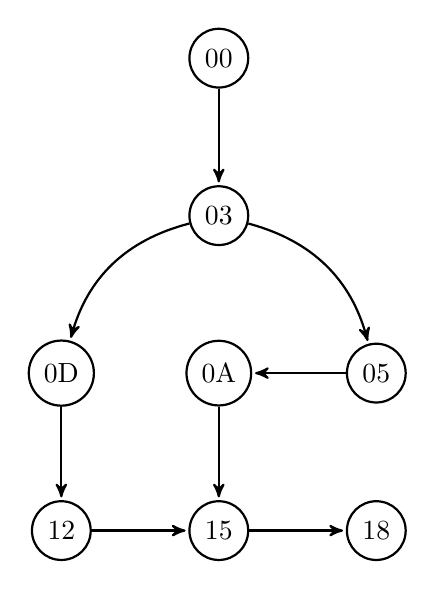
\begin{tikzpicture}
[->,>=stealth',shorten >=1pt,auto,node distance=2cm,thick,main node/.style={circle,draw}]

\node[main node] (00) {00};
\node[main node] (03) [below of=00] {03};
\node[main node] (0A) [below of=03] {0A};
\node[main node] (05) [right of=0A] {05};
\node[main node] (0D) [left of=0A] {0D};
\node[main node] (12) [below of=0D] {12};
\node[main node] (15) [below of=0A] {15};
\node[main node] (18) [right of=15] {18};


\path[every node/.style={font=\sffamily\small}]
    	(00) edge node [left] {} (03)
    	(03) edge [bend left] node [left] {} (05)
        	       edge [bend right] node[left] {} (0D)
    	(05) edge node [left] {} (0A)
    	(0D) edge node [left] {} (12)
    	(0A) edge node [left] {} (15)
	(15) edge node [left] {} (18)
	(12)edge node[left] {} (15)
	;
\end{tikzpicture}
\caption{Đồ thị luồng điều khiển được sinh ra từ tập tin ở Bảng \ref {table:tblexcfg}} 
\label{fig:imgexcfg}
\end{figure}

	\subsection{Những đòi hỏi trong quá trình hiện thực}

Đối với những tập tin nhị phân đơn giản, ta có thể dễ dàng quyết định được nút kế tiếp. Nhưng với những malware tinh vi, chúng sẽ có cách để ta không dễ dàng hiểu được ý định chúng sẽ làm gì, ra sao. Phương thức trên được gọi là làm rối mã (obfuscation). Một trong những cách điển hình có thể kể đến là nhảy gián tiếp (indirect jump -- thực hiện lệnh nhảy đến một giá trị không phải là hằng số như giá trị thanh ghi, giá trị ô nhớ...) và tự thay đổi mã (self-modification code -- trong quá trình thực thi sẽ tự ý thay đổi nội dung mã thực thi của chính mình).\\

Và BE-PUM đã được dựng lên để có thể chống lại việc làm rối mã này. Đó là điểm mạnh và là ưu thế vượt trội của BE-PUM so với các công cụ phân tích tĩnh mã thực thi khác như Jackstab, IDA Pro, Capstone, Unicorn, METASM, HOOPER bằng việc áp dụng phương pháp \textit{dynamic symbolic execution}.\\

\textit{Dynamic symbolic execution} là một phương pháp nhằm tính toán các giá trị thanh ghi và bộ nhớ ở một vị trí cụ thể, khi chúng ta không thể biết được điểm thực thi kế tiếp của chương trình là gì. Nhờ đó ta có thể giải quyết được các cách thức làm rối mã như nhảy gián tiếp, tự thay đổi mã như đã nói ở trên.\\

Để có thể tính toán được các giá trị thanh ghi cũng như bộ nhớ, ta cần xây dựng một hệ thống mô phỏng các câu lệnh mà một tập tin nhị phân thực hiện được. Các câu lệnh đó bao gồm 2 phần chính đó là \textit{hợp ngữ} và \textit{Windows API}.\\

\textbf{\textit{Đây là lý do chính hình thành nên đề tài luận văn này.}}

	\subsection{Ví dụ so sánh giữa BE-PUM và IDA Pro}

Đây là một ví du so sánh giữa BE-PUM và công cụ dịch ngược điển hình, rất nổi tiếng khác đó là IDA Pro, để cho thấy rõ được điểm mạnh và sự khác biệt của BE-PUM so với các công cụ khác.

\begin{longtable}{ | m{3cm} | m{5cm} | }
	\hline
Địa chỉ câu lệnh & Nội dung câu lệnh\\
	\hline
	\hline
0x00401000 & cmp eax, 0 \\
	\hline
0x00401003	& jne 0x00401015 \\
	\hline
0x00401005 & call 0x00401011 \\

	\hline
0x0040100a & add eax, 09h \\
	\hline
0x0040100d & inc eax \\
	\hline
0x0040100e & inc eax \\
	\hline
0x0040100f & jmp eax \\

	\hline
0x00401015 & push 0 \\
	\hline
0x00401017 & call  0x0040101c\\
	\hline
0x0040101c & jmp ExitProcess\\

	\hline
0x00401011 & mov eax, ss:[esp] \\
	\hline
0x00401014 & ret \\
	\hline

\caption{Nội dung của một tập tin nhị phân dưới dạng hợp ngữ (2)}
\label{table:tblAsmEx2}
\end{longtable}


\newpage

Nhìn vào đoạn mã ở Bảng \ref{table:tblAsmEx2}, ta nhận thấy tại địa chỉ \textit{0x0040100f} có thực hiện câu lệnh nhảy gián tiếp. Đối với các công cụ chạy trên mô hình phân tích tĩnh thì khi phân tích đến vị trí này, công cụ đó sẽ không thể tìm được điểm cần nhảy đến nữa và sẽ dừng việc phân tích ở đây lại. Ta có thể dễ dàng thấy được điều đó qua Hình \ref{fig:ModelReal} (b) ngay sau đây.\\

Nhưng đối với BE-PUM, một công cụ hỗ trợ cả phân tích tĩnh và phân tích động, thì tại điểm này, BE-PUM có thể tính toán được giá trị cần nhảy đến và dễ dàng tìm được điểm đích cần xử lý tiếp theo. Hình \ref{fig:ModelReal} (a) đã miêu tả rõ ràng được điều đó qua việc nút \textit{0x0040100f} đã liên thông đến nút cần xử lý là \textit{0x00401015}.

\newpage

\begin{figure}[H]
\centering
\begin{tabular}[c]{cc}
	\subfloat[BE-PUM]
	{
		\label{fig:BEPUMReal}
		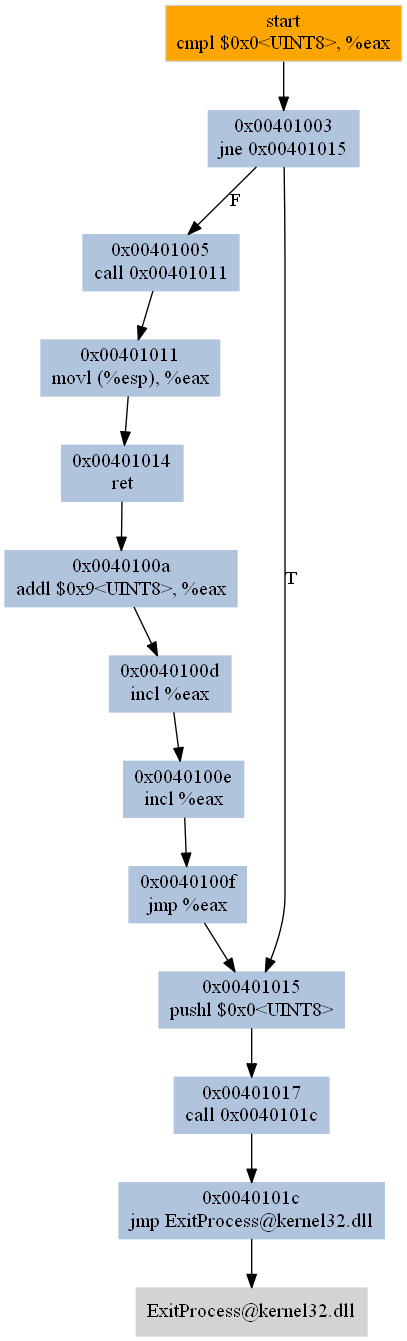
\includegraphics[width=0.4\textwidth]{bepum_sample}
    }
    &
	\subfloat[IDA Pro]
	{
		\label{fig:IDAReal}
        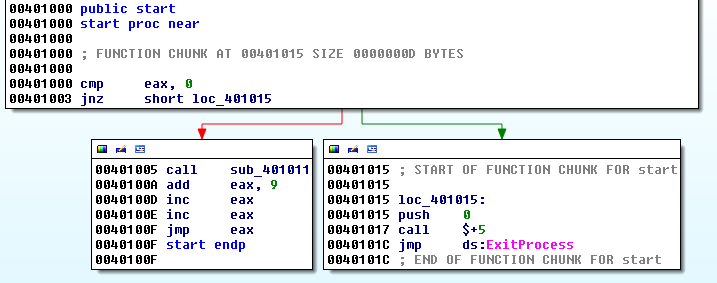
\includegraphics[width=0.6\textwidth]{ida_sample}
	}
\end{tabular}
\caption{Mô hình của BE-PUM và IDA Pro được sinh ra từ đoạn mã ở Bảng \ref {table:tblAsmEx2}}
\label{fig:ModelReal}
\end{figure}

\section{Tổng quan về hợp ngữ}
Ngôn ngữ assembly (hay hợp ngữ) là ngôn ngữ cấp thấp được biên dịch để thực thi một chương trình nào đó. Ngôn ngữ assembly có tính gợi nhớ, mỗi câu lệnh thực thi một chức năng, hay nhiệm vụ riêng biệt tương ứng với một lệnh yêu cầu máy thực thi. \\

Các chương trình sau khi biên dịch ra thành nhiều dạng file khác nhau để thực thi. Mỗi chương trình được biên dịch thành ngôn ngữ assembly trước khi biên dịch qua ngôn ngữ máy để máy hiểu và thực thi câu lệnh. Khi biên dịch qua mã assembly, đọc đoạn mã assembly để phân tích xem chương trình này có phải là virus máy tính không, có những hành vi bất thường từ đó xem xét đưa ra kết quả chương trình này có an toàn với máy tính.

\section {Tổng quan về Windows API}

Với tên gọi đầy đủ là Microsoft Windows application programming interface, đôi lúc được gọi một cách ngắn gọn là WinAPI, đây là một bộ giao diện lập trình ứng dụng (API) lõi có sẵn trong hệ điều hành Microsoft Windows (hay thường được gọi ngắn gọn là Windows).\\

Windows API là tên gọi chung của những dự án được triển khai cho những nền tảng khác nhau được áp dụng trong hệ điều hành Windows; mà thông thường chúng có những tên gọi riêng. Một số tên gọi và mô tả cho những phiên bản xin được trình bày trong Bảng \ref{table:tblwapiver}.\\

\newpage

\begin{longtable}{ | m{3cm} | m{11cm} | }
	\hline
Tên của phiên bản Windows API & Mô tả \\
	\hline
	\hline
Win16 & Đây là tên gọi bộ API đầu tiên có trong phiên bản Microsoft Windows 16-bit. Thuở ban đầu bộ API này có tên gọi là “Windows API”, nhưng sau khi phiên bản kế tiếp là Win32 ra đời, nó được đổi tên thành Win16. Lúc này các chức năng của Win16 API chủ yếu nằm trong các tập tin lõi của hệ điều hành như kernel.exe (hoặc krnl286.exe hoặc krnl386.exe), user.exe và gdi.exe. Dù rằng phần mở rộng là exe, nhưng thực tế đây là các thư viện liên kết động. \\
	\hline
Win32 & Đây là tên gọi cho bộ Windows API trong phiên bản Windows 32-bit, được giới thiệu lần đầu cùng hệ điều hành Windows NT. Các chức năng của Win32 API cũng bao gồm cả những chức năng của Win16 API, nhưng khác với phiên bản trước, chúng được đóng gói trong các tập tin DLL; trong đó có thể kể đến những tập tin DLL cốt lõi của Win32 API như: kernel32.dll, user32.dll, và gdi32.dll. \\
	\hline
Win64 & Đây là một biến thể sau đó của bộ API được hiện thực trong nền tảng Windows 64-bit. Cả chương trình 32-bit hoặc 64-bit đều có thể được biên dịch với cùng một mã nền duy nhất, dù rằng một số API trong Win32 đã được thay thế và loại bỏ. Tất cả con trỏ trong phiên bản này mặc định là 64-bit, do đó cần kiểm tra khả năng tương thích trong mã nguồn và viết lại nếu cần thiết. \\
	\hline

\caption[Một số phiên bản chính của Windows API]{Một số phiên bản chính của Windows API}
\label{table:tblwapiver}
\end{longtable}

\section{Mục tiêu đề tài}

Trong phạm vi của đề tài luận tốt nghiệp, mục tiêu nhắm tới là phát triển hệ thống xử lý các câu lệnh hợp ngữ và Windows API cho BE-PUM.\\

Với số lượng các API rất lớn hiện có trong hệ điều hành Windows, hiện tại đề tài đang tập trung vào xử lý các API ở phiên bản Win32 API, do hầu hết các phần mềm độc hại mà BE-PUM hướng tới vẫn đang dùng bộ API này; với sự ưu tiên từng bước xây dựng cho các API được dùng phổ biến trước.\\

Bên cạnh việc nhận thông tin đầu vào từ vùng nhớ đã được xây dựng của BE-PUM và trả về kết quả sau khi gọi API vào đúng địa chỉ cần thiết, điều quan trọng là phải đảm bảo không gây ngắt quãng cũng như tránh nguy hại hệ thống đang chạy. Và như vậy với những tương tác vật lý từ lời gọi API (bộ lưu trữ máy tính, cơ sở dữ liệu registry…) hay tương tác người dùng (API tạo cửa sổ message box, lệnh cho một thread “ngủ đông” trong một khoảng thời gian,…) cần được kiểm soát để không làm ảnh hưởng tới kết quả thực thi của BE-PUM.\\

\textit{Lưu ý: do nội dung đề tài tập trung vào xử lý cho Win32 API, nên kể từ đây, khi báo cáo nhắc đến Windows API tức là nói đến Win32 API.}\\

Việc hiện thực các câu lệnh hợp ngữ góp phần phân tích một số loại malware đang nghiên cứu. Dựa trên một số bộ malware hiện nay và những câu lệnh phổ biến thường gặp, BE-PUM sẽ hỗ trợ tốt công việc phân tích đúng môi trường làm việc của từng câu lệnh từ đó xác định chính xác và phân tính đúng các kỹ thuật mà malware đang tiến hành.

\newpage
\section{Giới hạn đề tài}

Trong phạm vi của đề tài luận văn tốt nghiệp, mục tiêu nhắm tới là hiện thực các câu lệnh hợp ngữ và Windows API với số lượng đạt mức như sau:

\begin{itemize}
  \item Số lượng câu lệnh hợp ngữ được hỗ trợ đạt khoảng 250 câu lệnh.
  \item Số lượng câu lệnh Windows API được hỗ trợ đạt khoảng 400 câu lệnh.
\end{itemize}

\section{Cấu trúc của báo cáo}

Bài báo cáo này bao gồm những đề mục sau đây:

\begin{description}
  	\item[Chương 1] \hfill \\
	Giới thiệu tổng quan về BE-PUM, điểm mạnh của công vụ này và so sánh với công cụ khác, những đòi hỏi trong quá trình hiện thực công cụ và yếu tố quyết  định để cho ra đề tài này; dẫn nhập về hợp ngữ assembly, dẫn nhập về Windows API, các thành phần sẽ được áp dụng để phát triển cho BE-PUM; nêu ra mục tiêu của đề tài và giới hạn trong phạm vi luận văn tốt nghiệp. \\
 	\item[Chương 2] \hfill \\
	Đem đến những cái nhìn về những vấn đề đã và đang được lưu tâm khi thực hiện đề tài này; sự phổ biến của Windows API trong những phần mềm độc hại để thấy sự cần thiết của việc xây dựng một bộ xử lý Windows API cho BE-PUM; những khó khăn khi thực hiện điều đó và giải pháp cho vấn đề. Đông thời phân tích vấn đề đặt ra là hiện thực các câu lệnh trong hợp ngữ assembly, giải thích tại sao sử dụng ngôn ngữ assembly để tiến hành phân tích chương trình.\\
	\item[Chương 3] \hfill \\
	Trình bày những kiến thức cần thiết cho quá trình thực hiện đề tài; từ những kiến thức phải nắm được về hệ thống BE-PUM do đây là một đề tài làm việc dựa trên đó; và mỗi khi làm việc với một thư viện bất kỳ, đòi hỏi ta phải tìm hiểu cách thức làm việc với thư viện đó và cả những kiến thức cần thiết do bộ thư viện ấy yêu cầu. Đồng thời cũng trình bày các kiến thức cơ bản về hợp ngữ assembly, từ đó có cái nhìn tổng quan về assembly để tiến hành xây dựng chương trình BE-PUM. \\
	\item[Chương 4] \hfill \\
	Mỗi chương trình bất kỳ đều cần một thiết kế tốt để giúp cho việc xây dựng dễ dàng và quy chuẩn hơn. Mục này sẽ trình bày cách mà bộ xử lý Windows API đã được hiện thực để tương tai sau này có thể dễ dàng sửa chữa, bảo trì và bổ sung thêm vào kiến trúc đó. Để hiểu rõ cấu chương trình mô phỏng câu lệnh assembly, sơ đồ class trình bày trong chương này thể hiện được mối quan hệ giữa các class, cấu trúc của chương trình BE-PUM được phát triển dựa trên dự án JakStab, giới thiệu các class quan trọng của chương trình BE-PUM.\\
	\item[Chương 5] \hfill \\
	 Trình bày và phân tích, so sánh với các công cụ khác về kết quả mà đề tài đã đạt được sau khi tiến hành thực hiện công việc, kết quả tổng thể mà bộ xử lý đã được đóng góp để hỗ trợ cho hệ thống BE-PUM.\\
	\item[Chương 6] \hfill \\
	 Sau khi có được những kết quả ở thời điểm hiện tại của quá trình thực hiện đề tài, chương cuối này sẽ trình bày về những phương hướng cần tiếp tục phát triển trong tương lai đối với đề tài hiện tại.\\
	\item[Phụ Lục] \hfill \\
	 Liệt kê về những tài liệu và nguồn tham khảo có liên quan đến đề tài này.\\
\end{description}


\chapter{Phân Tích Vấn Đề}
\section{BE-PUM và những khó khăn}

	\subsection{Mục tiêu hướng đến của BE-PUM}

	\subsection{Các hướng tiếp cận}

	\subsection{Mô hình luồng điều khiển}

	\subsection{Những đòi hỏi trong quá trình hiện thực}

%%%%%%%%%%%%%%%%%%%%%%%%%%%%%%%%%%%%%%%%%%%%%%%%%%%%%
%%%%%%%%%%%%%%%%%%%%%%%%%%%%%%%%%%%%%%%%%%%%%%%%%%%%%
%%%%%%%%%%%%%%%%%%%%%%%%%%%%%%%%%%%%%%%%%%%%%%%%%%%%%

\section{Các câu lệnh hợp ngữ}
  \subsection{Assembly ngôn ngữ dùng để phân tích }
  Với các chương trình cần được phân tích, việc biết mã nguồn của chương trình là một điều rất khó khăn và hầu như là không thể biết được do đó để phân tích chương trình, BE-PUM dich ngược chương trình cần phân tích từ mã chương trình đó, dựa vào các opcode để chuyển sang mã assembly để có thể đọc được và hiểu được chương trình đang thực thi gì?\\

Tại sao lại chọn mã assembly để phân tích? Vì lý do không thể tìm được mã nguồn của chương trình cần phân tích, để tiến hành dịch ngược, và trên cơ sở mọi chương trình thực thi đều phải biên dịch qua ngôn ngữ máy là mã nhị phần. Từ đó quyết định chọn ngôn ngữ assembly là ngôn ngữ cấp thấp nhưng vẫn có thể đọc hiểu và phân tích. Từ đó, dựa trên đoạn mã assembly của chương trình cần phân tích, BE-PUM tiến hành phân tích đoạn mã assembly để trả lời câu hỏi “Chương trình này có phải là virus hay không?”\\

  \subsection{BE-PUM và Assembly}
  Hợp ngữ assembly là một ngôn ngữ lập trình cấp thấp. Trên thực tế đã có rất nhiều chương trình được viết bằng ngôn ngữ assembly được áp dụng cho những chiếc máy tính đầu tiên. Công việc lập trình bằng ngôn ngữ assembly rất cực nhọc, dễ xảy ra lỗi trong quá trình lập trình và tốn rất nhiều chi phi, công sức và thời gian. Các chương trình viết bằng hợp ngữ phụ thuộc rất nhiều vào kiến trúc máy tính của nó, và trong phạm vi của công cụ BE-PUM, dựa trên kiến trúc X86 của Microsoft Windows để tiến hành phân tích chương trình.\\

Hợp ngữ assembly là tập hợp các câu lệnh gợi nhớ giúp người lập trình có thể hiểu được, là một ngôn ngữ cấp thấp nhưng vẫn có thể dễ đọc. Số lượng câu lênh assembly là khá nhiều do đó trong qua trình xây dựng công cụ phân tich BE-PUM tập trung vào những câu lệnh mà virus thường hay sử dụng và hiện thực thêm các câu lệnh để hỗ trợ trong quá trình phân tích virus.\\

BE-PUM là một dự án được phát triển lên từ dự án JakStab và được viết hoàn toàn bằng ngôn ngữ JAVA. Việc hiện thực câu lệnh assembly trên JAVA có đôi chút khó khăn khi không có thư viện hỗ trợ, với mỗi câu lệnh assembly có biến môi trường khác nhau, nhiệm vụ khác nhau vì vậy để hiện thực một câu lệnh hoàn chỉnh cần phải có tài liệu tham khảo, có ví dụ từng trường hợp cụ thể, tránh sai xót hoặc xử lý thiếu trường hợp. Việc tìm tài liệu với từng câu lệnh cũng gặp đôi chút khó khăn khi tài liệu một số câu lệnh rất ít. Do đó để hạn chế những thiếu xót, các câu lệnh assemby thường được kiểm tra, nếu có trường hợp sai xảy ra sẽ được tìm hiểu và khắc phục.\\

  \subsection{Phân tích Assembly trong BE-PUM}
  Mục đích của chương trình Be-Pum đặt ra trả lời câu hỏi “Chương trình này có phải là virus hay không?”. Để trả lời câu hỏi này có rất nhiều cách khác nhau để hiện thực chương trình, Be-Pum dựa trên phân tích hành vi của chương trình để trả lời vấn đề trên. Phân tích mã assembly là một trong những bước đầu để trả lời câu hỏi đó. Assembly là ngôn ngữ cấp thấp nhưng người lập trình vẫn có thể đọc được nó, và mọi chương trình khi thực thi đều có thể biên dịch ra mã assembly. Do đó, dựa vào hành vi của chương trình và tiến hành phân tích mã assembly mà có thể đưa ra kết luận.\\

Để giải quyết vấn đề hỗ trợ, phân tích từng câu lệnh của assembly, BE-PUM tiến hành xây dựng các class để tiến hành phân tích, hiện thực câu lệnh. Chia nhỏ vấn đề của từng câu lệnh thành các hàm trong từng class để hiện thực. Việc chia nhỏ vấn đề có thể giải quyết những câu lệnh có tính lặp lại, xử lý cùng một tính năng hay mục đích nào đó của câu lệnh. Giúp quản lý tốt hơn về hiện thực câu lệnh.\\

Có rất nhiều bước để hoàn thành chương trình Be-Pum, trong đó đọc hiểu mã assembly đầu vào là một trong những bước cơ bản. Có rất nhiều câu lệnh assembly mà BE-PUM chưa hỗ trợ, do đó cần đặt ra nhiệm vụ là hiện thực các câu lệnh assembly trong BE-PUM. Tính tới thời điểm hiện nay, Be-Pum đã hiện thực 200 câu lệnh thực thi số nguyên và 65 câu lệnh thực thi số thực và đã được kiểm tra. \\ 

%%%%%%%%%%%%%%%%%%%%%%%%%%%%%%%%%%%%%%%%%%%%%%%%%%%%%
%%%%%%%%%%%%%%%%%%%%%%%%%%%%%%%%%%%%%%%%%%%%%%%%%%%%%
%%%%%%%%%%%%%%%%%%%%%%%%%%%%%%%%%%%%%%%%%%%%%%%%%%%%%

\section{Windows API}
	\subsection{Windows API trong những phần mềm độc hại}

Để cung cấp sức mạnh và sự tiện lợi cho lập trình viên trong việc viết ứng dụng chạy trên hệ điều hành Windows, các API trong bộ Windows API mở ra nhiều cách thức nhanh chóng và mạnh mẽ cho lập trình viên trong việc tương tác với hệ thống.\\

Và vấn đề gì cũng có hai mặt của nó, sự hỗ trợ mạnh mẽ đó cũng là con đường đơn giản để các tin tặc áp dụng vào việc xây dựng nên các phương pháp tấn công, cũng như cho ra đời những phần mềm nguy hại (malware), để lại bao hậu quả xấu cho hệ thống máy vi tính trên toàn cầu.\\

Trong quá trình xây dựng BE-PUM và qua việc phân tích hàng ngàn mẫu malware chạy trên môi trường Windows được phát tán ở khắp nơi trên thế giới, hầu hết những mẫu malware trên đều áp dụng lời gọi Windows API vào cách thức tấn công của chúng. Những phương pháp tấn công phổ biến như SEH hay phương pháp chống phát hiện đều có sự tồn tại của Windows API trong đó.\\

Do đó, việc xây dựng một bộ công cụ xử lý những thông tin trả về từ Windows API là rất cần thiết cho việc phát triển hệ thống BE-PUM, một hệ thống tập trung vào phân tích mã nhị phân của malware.\\


%%%%%%%%%%%%%%%%%%%%%%%%%%%%%%%%%%%%%%%%%%%%%%%%%%%%%


	\subsection{BE-PUM và Windows API}

Mã nguồn của những API trong bộ Windows API được tập đoàn Microsoft giữ kín và không hề công bố. Chỉ có những đặc tả và hướng dẫn sử dụng được Microsoft phổ biến rộng rãi cho lập trình viên. Nghĩa rằng ta chỉ có thể biết được đầu vào của lời gọi và mong muốn đầu ra sẽ như ý, chứ không thể nắm rõ lô-gíc xử lý bên trong của chúng. Điều đó khiến cho việc xử lý đúng đắn một cách tổng quát đối với mọi đầu vào của mỗi API bằng cách viết lại bộ mã xử lý tương ứng của chúng vào trong BE-PUM dường như trở nên không thể.\\

Hướng tiếp cận hiện tại là tiến hành lấy nội dung bộ nhớ, nội dung các đối số nằm trên stack bên trong BE-PUM và tiến hành gọi thực sự với Windows API, nhận kết quả trả về và nạp lại vào trong BE-PUM để tiếp tục tiến hành phân tích các câu lệnh tiếp theo.\\

BE-PUM là một dự án được phát triển lên từ nhân của dự án JakStab và được viết hoàn toàn trên ngôn ngữ lập trình Java. Với Windows API thì lại là một câu chuyện hoàn toàn khác, Windows API được phát triển chủ yếu tập trung vào ngôn ngữ lập trình C kèm với các mô tả và cấu trúc dữ liệu được viết trên đó. Thêm lần nữa, việc hiện thực ý tưởng gọi để lấy kết quả Windows API từ trong lòng BE-PUM gặp nhiều khó khăn. Đặc biệt là việc ánh xạ các dữ liệu kiểu cấu trúc giữa hai thành phần trên cũng là một trăn trở.\\

Vì những lý do trên, cần tìm hiểu một cách thức giải quyết vấn đề nhanh chóng và đơn giản hơn bằng một bộ công cụ nào đó để xử lý rào cản ngôn ngữ giữa Java và C. Thêm vào đó, bộ công cụ này cũng cần có tính linh hoạt và mềm dẻo để cho việc phát triển về sau được dễ dàng.\\


%%%%%%%%%%%%%%%%%%%%%%%%%%%%%%%%%%%%%%%%%%%%%%%%%%%%%


	\subsection{Truy xuất Windows API bên trong BE-PUM thông qua JNA}

Vấn đề trên được giải quyết thông qua bộ thư viện Java Native Access (JNA).\\

Java Native Access là một thư viện được cộng đồng phát triển, nhằm giúp cho các chương trình được viết bằng ngôn ngữ lập trình Java dễ dàng truy cập vào các thư viện native shared mà không cần thông qua Java Native Interface. Thiết kế của JNA cũng cung cấp khả năng này mà không cần bỏ ra nhiều công sức.\\

Với khả năng ánh xạ dễ dàng giao diện lập trình giữa hai ngôn ngữ Java và C; bao gồm ánh xạ tên hàm, kiểu dữ liệu trả về, kiểu dữ liệu của các thông số đầu vào; từ những kiểu dữ liệu cơ bản đến những kiểu dữ liệu cấu trúc và kể cả con trỏ; đó là những ưu điểm để lựa chọn JNA áp dụng vào trong việc giải quyết yêu cầu của đề tài nêu trên.

\chapter{Kiến Thức Nền}
\section{Làm việc với BE-PUM}

Trong BE-PUM có xây dựng một hệ thống mô tả môi trường làm việc tương tự như trên một hệ thống máy tính khởi chạy ngoài thực tế; chúng bao gồm các thành phần chính mà đề tài sẽ ảnh hưởng đến như sau:

\begin{itemize}
\item 	\textbf{Chồng (stack)} là một đơn vị dùng để lưu trữ giá trị theo nguyên tắc xếp chồng lên nhau, hoạt động theo nguyên lý vào sau ra trước (Last In First Out (LIFO)). Nó được dùng với nhiều mục đích khác nhau, ví dụ như để ghi nhận địa chỉ cần trở về khi thực hiện gọi một chương trình con, hay để ghi nhận các giá trị của các tham số truyền vào khi gọi một hàm Windows API.\\

\item 	\textbf{Bộ nhớ (memory)} dùng để lưu trữ toàn bộ giá trị của các vùng nhớ mà chương trình đang làm việc. Windows API cũng có khả năng tương tác với phần này; do vậy, đòi hỏi khi xây dựng xử lý API cần đảm bảo kết quả chính xác cho thành phần này.\\

\item 	\textbf{Thanh ghi (register)} là một vùng nhớ có dung lượng nhỏ nhưng lại có khả năng truy xuất rất nhanh, chúng được dùng để làm vùng nhớ tạm, trung gian cho các câu lệnh chạy trong hệ thống. Mỗi khi gọi một hàm bất kỳ, nếu như kiểu trả về khác void thì giá trị trả về sẽ được lưu trữ vào thanh ghi EAX.\\
\end{itemize}


\section{Các câu lệnh hợp ngữ}

	\subsection{Assembly}
	
		\subsubsection{Bộ nhớ assembly}	
		 Biến và hằng trong assembly có tính chất và mục đích sử dụng khác nhau. Thông qua các câu lệnh liên kết chặn chẽ với bộ nhớ là các thanh ghi bộ nhớ, trạng thai, các cờ được đánh dấu mà thông qua đó để thực thi chương trình.\\

		Các thanh ghi bộ nhớ:		
		\begin{center}
			\begin{figure}[htp]
				\begin{center}
					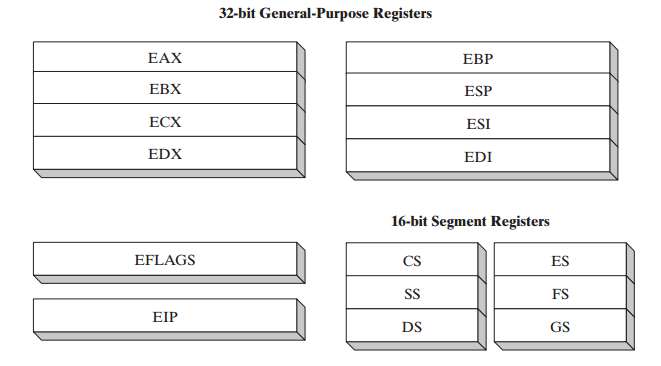
\includegraphics[scale=0.5]{ThanhGhi.png}
				\end{center}
				\caption{Thanh ghi (trính dẫn hình ảnh trong sách Assembly Language)}
				\label{fig:Flow}
			\end{figure}
		\end{center}
		
		Trong đó các thanh ghi General-Purpose gồm những thanh ghi có số bit nhỏ hơn:	
		\begin{center}
			\begin{figure}[htp]
				\begin{center}
					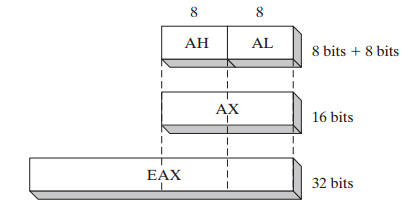
\includegraphics[scale=0.5]{ThanhGhi32bit.png}
				\end{center}
				\caption{Thanh ghi (trính dẫn hình ảnh trong sách Assembly Language)}
				\label{fig:Flow}
			\end{figure}
		\end{center}
		
		Ví dụ: thanh ghi EAX(32 bit địa chỉ) có thể được chia ra gồm thanh ghi AX(16 bit địa chỉ). Thanh ghi AX tiếp tục chia địa chỉ thành AH(8 bit) và AL(8 bit). Việc chia địa chỉ như thế giúp tối ưu bộ nhớ khi sử dụng.\\
		\begin{longtable}{ | m{3cm} | m{3cm} | m{3cm}  | m{3cm}| }
			\hline
				32 Bit & 16 Bit & 8Bit & 8 Bit\\
			\hline
			\hline
				EAX & AX	& AH	 & AL\\
			\hline			
				EBX & BX	& BH	 & BL\\
			\hline		
				ECX & CX	& CH	 & CL\\		
			\hline
				EDX & DX	& DH	 & DL\\
			\hline
			\caption{Bảng chia bộ nhớ 32-bit, 16-bit, 8-bit}
			\label{table:tbthanhghi}
		\end{longtable}
		
			Đối với một số thanh ghi có 32-bit địa chỉ có thể chia ra 16-bit địa chỉ, không thể chia nhỏ hơn. Bảng chi bộ nhơ thanh ghi có thể chia ra 16-bit địa chỉ.\\
			\begin{longtable}{ | m{3cm} | m{3cm} | }
			\hline
				32 Bit & 16 Bit\\
			\hline
			\hline
				ESI & SI\\
			\hline			
				EDI & DI\\
			\hline		
				EBP & BP\\		
			\hline
				ESX & SP\\
			\hline
			\caption{Bảng chia bộ nhớ 32-bit,16-bit}
			\label{table:tbthanhghi}
		\end{longtable}
		
	Mỗi thanh ghi có một chức năng khác nhau: 
\begin{itemize}
	\renewcommand{\labelitemi}{\textbullet}
	\item	EAX: thường được sử dụng trong các phép tính số học: cộng, trừ, nhân, chia, các phép toán logic, chuyển dữ liệu.
	\item EBX: được sử dụng như thanh ghi địa chỉ .
\item	ECX: được sử dụng trong các phép lặp, chuyển bit địa chỉ, xoay bit địa chỉ.
\item	EDX: thường được dùng để lưu dữ liệu, kết hợp vơi thanh ghi EAX thực hiện các phép toán nhân, cộng.
\item	ESP: luôn trỏ thới địa chỉ đỉnh stack hiện thời.
\item	EBP: thanh ghi dùng để truy cập giá trị, nhập dữ liệu stack. Khác với thanh ghi ESP, thanh ghi EBP còn được sử dụng để truy cập trong các đoạn chương trình khác nhau.
\item	EIP: thanh ghi con trỏ chỉ dẫn, giá trị của thanh ghi không thể thay đổi một các trực tiếp, chỉ thay đổi khi trỏ tới câu lệnh tiếp theo. Thanh ghi EIP lưu giá trị trỏ tơi của câu lệnh tiếp theo sẽ được gọi. 
\item	ESI, EDI: thanh ghi chỉ số nguồn và chỉ số đích thường được dùng trong các thao tác, xử lý mảng và chuỗi.
\end{itemize}	
	
	Thanh ghi EFLAGS bao gồm các chuỗi nhị phân được điều khiển bởi CPU hoặc phản ánh một số phép toán của CPU. Trạng thái của CPU. Bao gồm 8 cờ hiệu với mỗi loại cờ có chức năng khác nhau:
\begin{itemize}
	\renewcommand{\labelitemi}{\textbullet}		
		\item CF(Carry Flag cờ nhớ): cờ được bật khi phép tính có nhớ bit.
		\item ZF(Zero Flag cờ 0): cờ được bật khi phép tính vừa thực hiện là 0.
\item SF(Sign Flag cờ dấu): cờ này được bật khi kết quả thực phép tính có bit dấu.
\item	OF(Overflow Flag cờ tràn): cờ được bật khi kết quả thực hiện phép tính bị tràn số học.
\item	PF(Parity Flag cờ chẵn lẽ): cờ được bật khi kết quả của phép tính có chẵn bit 1.
\item	AF(Auxilary Flag cờ nhớ phụ): cờ được bật khi phép tính được thực hiện có sử dụng bit nhớ phụ.
\item IF(Interrupt Flag cờ ngắt): cờ được bật khi có thông báo cho phép ngắt xảy ra.
\item DF(Direction Flag cờ hướng): cờ được bật và sử dụng khi thao tác với mảng và chuỗi, sử dụng để giảm chỉ số tự động thi thao tác.
\end{itemize}	

		\subsubsection{Câu lệnh assembly}
		Một câu lệnh assembly có cú pháp đầy đủ như sau: 
		 \begin{center}		 
			\fontshape{it}  
			\selectfont
		 	$[ $ Nhãn lệnh: $]$  	$<$ Tên lệnh $<$ 	$[$ Các toán hạng $]$	$[$ ;lời chú thích $]$ \\
		 \end{center}			
		Trong đó:
		
		\begin{itemize}
		\renewcommand{\labelitemi}{\textbullet}		
		\item $[$ Nhãn lệnh: $]$  là một chuỗi ký tự kết thúc bằng dâu “:”, được thanh thế cho địa chỉ câu lệnh, được sử dụng trong câu lệnh If, else hoặc cần gọi thay bằng địa chỉ câu lệnh. Trong một chương trình không thể có hai nhãn lệnh trùng tên, tên nhãn lệnh không được trùng với tên thủ tục.
		\item $<$Tên lệnh $>$là một trong số những lệnh gợi nhớ của mã assembly, không phân biệt chữ hoa, chữ thường. Mỗi dòng lệnh chỉ đảm nhận một câu lệnh, mỗi câu lệnh phải được đặt trên một dòng.
		\item $[$Các toán hạng$]$ là các đối tượng mà câu lệnh sẽ tác động vào. Tùy theo từng câu lênh mà có 0 toán hạng, 1 toán hạng, 2 toán hạng, 3 toán hạng. Toán hạng đầu tiên gọi là toán hạng đích, toán hạng thứ 2 gọi là toán hạng nguồn. Với câu lệnh có 3 toán hạng thì chỉ có 1 toán hạng đích trong câu lệnh đó. 
		\item $[$; lời giải thích$]$ khi biên dịch thì lời giải thích không được biên dịch sang mã máy, chỉ có tác dụng với người đọc chương trình. Giúp người đọc dễ hiểu các câu lệnh.
		\end{itemize}

	Ví dụ 1: xét câu lệnh sau đây: 
	 \begin{center}		 
		VD1: mov ax, bx	;lưu giá trị thanh ghi ax từ thanh ghi bx
	\end{center}
	Trong đó:
	\begin{itemize}
		\renewcommand{\labelitemi}{\textbullet}			
	  \item	VD1 : là chuỗi ký tự nhãn lệnh.
	\item	mov: tên lệnh với chức năng lưu giá trị đích(ax) từ giá trị nguồn (bx).
	\item	ax, bx: các toán hạng, trong trường hợp này là các thanh ghi bộ nhớ 16 bit.
	\item $;$ lưu giá trị thanh ghi ax từ thanh ghi bx : lời giải thích, chú thích thêm.
	\end{itemize}
	
	Xem các câu lệnh sau đây:
	\begin{itemize}
	\renewcommand{\labelitemi}{\textbullet}		
	\item  NOT	: đây là câu lệnh không có toán hạng.
	\item	Mov ax, bh: câu lệnh này có 2 toán hạng ax (toán hạng đích) thanh ghi 16 bit, bh (toán hạng nguồn) thanh ghi 8 bit.
	\item	Add ah, sqt: câu lệnh này có 2 toán hạng ah (toán hạng đích) thanh ghi 8 bit, sqt (toán hạng nguồn) một biến được gán trước có kiểu dữ liệu là byte.
	\item	Mov ax, [SI]: câu lệnh này có 2 toán hạng ax (toán hạng đích) thanh ghi 16 bit, [SI] (toán hạng nguồn) là một ô nhớ.
	\item	Imul ax, bx, 10: câu lệnh này có 3 toán hạng ax (toán hạng đích) thanh ghi 16 bit, bx (toán hạng nguồn) thanh ghi 16 bit, và một hằng số (10).
	\end{itemize}

	Câu lệnh Imul có tới 3 toán hạng, toán hạng đích (ax) sẽ được lưu kết quả của phép nhân từ toán hạng nguồn (bx) nhân với hằng số (10: tức toán hạng thứ 3).\\
	Bảng ký hiệu toán hạng:
	\begin{longtable}{ | m{3cm} | m{12cm} | }
			\hline
				Toán hạng & 16 Mô tả\\
			\hline
			\hline
				reg8 & Thanh ghi có 8 bit địa chỉ: AH, AL, BH, BL, CH, CL, DH, DL \\
			\hline			
				reg16& Thanh ghi có 16 bit địa chỉ: AX, BX, CX, DX, SI, DI, SP, BP\\
			\hline		
				reg32& Thanh ghi có 32 bit địa chỉ: EAX, EBX, ECX, EDX, ESI, EDI, ESP, EB\\
			\hline	
				reg&	Bất kỳ thanh ghi nào\\
			\hline	
				sreg & Thanh ghi segment có 16 bit địa chỉ: CS, DS, SS, ES, FS, GS\\
			\hline	
				imm	&8- , 16-, hoặc 32- bit giá trị được truyền vào\\
			\hline	
				imm8	& Giá trị hằng số truyền vào kiểu byte 8-bit\\
			\hline	
				imm16	& Giá trị hằng số truyền vào kiểu word 16-bit\\
			\hline	
				imm32&	Giá trị hằng số truyền vào kiểu doubleword 32-bit\\
			\hline	
				reg/mem8& Toán hạng 8 bit, có thể là thanh ghi có 8-bit địa chỉ hoặc bộ nhớ byte\\
			\hline	
				reg/mem16&	Toán hạng 16 bit, có thể là thanh ghi có 16-bit địa chỉ hoặc bộ nhớ word\\
			\hline	
				reg/mem32	& Toán hạng 32 bit, có thể là thanh ghi có 32-bit địa chỉ hoặc bộ nhớ doubleword\\
			\hline	
				mem	& Bất kỳ bộ nhớ 8-, 16-, 32- bit\\
		\hline	
			\caption{Bảng ký hiệu toán hạng:}
			\label{table:tbkyhieu}
	\end{longtable}
	
		Phân tích câu lệnh mov: \\
		Cú pháp: 
		\begin{itemize}
			\renewcommand{\labelitemi}{\textbullet}	
			\item Mov [toán hạng đích], [toán hạng nguồn].
			\item	Mov reg/mem8, reg8
			\item Mov reg/mem16, reg16
			\item	Mov reg/mem32, reg32
			\item	Mov reg8, reg/mem8
			\item	Mov reg16, reg/mem16
			\item	Mov reg32, reg/mem32
			\item	Mov reg/mem16, sreg
			\item	Mov sreg, reg/mem16
			\item	Mov reg8, imm8
			\item	Mov reg16, imm16
			\item	Mov reg32, imm32
			\item	Mov reg/mem8, imm8
			\item	Mov reg/mem16, imm16
			\item	Mov reg/mem32, imm32	
		\end{itemize}
	
	Trong đó: 
	\begin{itemize}
		\renewcommand{\labelitemi}{\textbullet}	
			\item  $[$ Toán hạng đich$]$: có thể là thanh ghi (8 bit, 16 bit, 32 bit), ô nhớ (địa chỉ của ô nhớ) hay một biến nào đó.$[$Toán hạng đích$]$không thể là hằng số.
			\item $[$ Toán hạng nguồn $]$: có thể là hằng số, biến, thanh ghi, ô nhớ.
	\end{itemize}

	Xem ví dụ sau:
		\begin{itemize}
		\renewcommand{\labelitemi}{\textbullet}	
		\item	Mov ax, bx 		; đặt giá trị của thanh ghi bx vào ax.
		\item Mov ax, 5		; đặt giá trị 5 vào thanh ghi ax.
		\item	Mov bx, 5*3 		; đặt giá trị 5*3 vào thanh ghi bx.
		\item Mov DI, ‘A’		; đặt mã ASCII của ‘A’ vào thanh ghi DI
		\item Mov ch, var		; đặt giá trị của biến var kiểu byte vào thanh ghi ch.
		\item	Mov bh, 300		; giá trị không hợp lệ vì bh có kiểu byte giới hạn 255 nên không thể gán giá trị 300 vào bh.
		\item	Mov ch, ax		; giá trị không hợp lệ vì giá trị thanh ghi ax (16 bit) không thể gán giá trị vào thanh ghi ch (16 bit).  
		\end{itemize}

		\subsubsection{Tập giá trị}
		Khác với các ngôn ngữ lập trình khác, kiểu giá trị của assembly có đôi chút khác biệt, được tính theo bit, tùy theo yêu cầu sử dụng của người lập trình. \\
		Các kiểu dữ liệu:
		\begin{longtable}{ | m{3cm} | m{8cm} | }
			\hline
				Kiểu & Cách sử dụng\\
			\hline
			\hline
				BYTE & 	kiểu số nguyên 8-bit không dấu.\\
			\hline
				SBYTE	& kiểu số nguyên 8-bit có dấu.\\
			\hline
				WORD& 	kiểu số nguyên 16-bit không dấu.\\
			\hline
				SWORD	& kiểu số nguyên 16-bit có dấu.\\
			\hline
				DWORD& 	kiểu số nguyên 32-bit không dấu.\\
			\hline
				SDWORD& 	kiểu số nguyên 32-bit có dấu.\\
			\hline
				FWORD	& kiểu số nguyên 48-bit.\\
			\hline
				QWORD& 	kiểu số nguyên 64-bit\\
			\hline
				TBYTE& 	kiểu số nguyên 80-bit (10-byte).\\
			\hline
				REAL4& 	kiểu số thực 32-bit (4-byte) chuẩn IEEE.\\
			\hline
				REAL8& 	kiểu số thực 64-bit (8-byte) chuẩn IEEE.\\
			\hline
				REAL10& 	kiểu số thực 80-bit (10-byte) chuẩn IEEE.\\			
			\hline
					\caption{Bảng kiểu dữ liệu:}
					\label{table:tbkieudulieu}
		\end{longtable}
		
		Ngoài ra còn có một số ký hiệu kiểu số tự nhiên.
		\begin{longtable}{ | m{3cm} | m{6cm} | }
			\hline
				Kiểu & Cách sử dụng\\
			\hline
			\hline
				DB &	kiểu số nguyên 8-bit.\\
			\hline
				DW &	kiểu số nguyên 16-bit.\\
			\hline			
				DD &	kiểu số nguyên hoặc số thực 32-bit.\\
			\hline
				DQ	 &kiểu số nguyên hoặc số thực 64-bit.\\
			\hline
				DT	 &định nghĩa kiểu số nguyên 80-bit (10 byte).\\
			\hline
					\caption{Bảng ký hiệu kiểu số tự nhiên:}
					\label{table:tbkieudulieutn}
		\end{longtable}
		
		Trên cở sở các đơn vị dữ liệu được lưu trên kiến trúc X86, một byte tưng ứng với 8-bit, tưng tự word tưng ứng với 16-bit (2 byte), doubleword tưng ứng với 32-bit (4 byte), quadword tưng ứng với 64-bit (8 byte). Từ đó ta tính toán được phạm vi giới hạn số học của các kiểu số nguyên không dấu và có dấu: 
			\begin{longtable}{ | m{5cm} | m{6cm} | m{3cm} |}
			\hline
				Kiểu lưu trữ &	Phạm vi (từ thấp đến cao)&	Dung lượng\\
			\hline
			\hline
				Byte không dấu &	0 đến 255&	1 byte\\
			\hline
				Word không dấu	&0 đến 65,535&	2 bytes\\
			\hline
				Double word không dấu	 &0 đến 4,294,967,295&	4 bytes\\
			\hline
				Quadword không dấu	&0 đến 18,446,744,073,709,551,615&	8 bytes\\
			\hline
				\caption{Bảng phạm vi kiểu dữ liệu số không dấu}				
			\end{longtable}
		
			\begin{longtable}{ | m{5cm} | m{7cm} |}
			\hline
				Kiểu lưu trữ	& Phạm vi (từ thấp đến cao)\\
			\hline
			\hline
				Byte có dấu	& -128 đến +127\\
			\hline
				Word có dấu &	-32,768 đến +32,767\\
			\hline	
				Double word có dấu &	-2,147,483,648 đến +2,147,483,647\\
			\hline	
				Quadword có dấu	 & -9,223,372,036,854,775,808 đến +9,223,372,036,854,775,807 \\
			\hline
			\caption{Bảng phạm vi kiểu dữ liệu số có dấu}				
			\end{longtable}		
		
		\subsubsection{Kiếu giá trị}
		\subsubsection*{Hằng số}
		Kiểu hằng số nguyên được dùng trong hợp ngữ assembly là một chuỗi số đứng trước nó là dấu của số nguyên đó, tiếp theo là chuỗi số và cuối cùng là cơ số để xác định chuỗi số đó. Cú pháp của chuỗi số:		
		\begin{center}
			\fontshape{it}  
			\selectfont
		 	$[{+|-}]$ chuỗi số$ [$cơ số$]$
		\end{center}
	
	Cơ số là một trong những dạng cơ số dưới đây (không phân biệt chứ hoa hay chữ thường):
		\begin{itemize}
		\renewcommand{\labelitemi}{\textbullet}	
			\item	h	: Hexadecimal hệ cơ số 16
			\item	q/o	: Octal hệ cơ số 8
			\item	d	: Decimal hệ cơ số 10
			\item	b	: Binary hệ cơ số 2
		\end{itemize}			
	Nếu không có ký hiệu cơ số thì mặc định số đó là hệ cơ số 10. Dưới đây là một số ví dụ:
	\begin{itemize}
	\item	26		: 26 hệ cơ số 10
	\item	26d		: 26 hệ cơ số 10
	\item	11010011b	: 11010011 hệ cơ số 2
	\item	42q		: 42 hệ cơ số 8
	\item	42o		: 42 hệ cơ số 8
	\item	1Ah		: 1A hệ cơ số 16
	\end{itemize}	
	
	\subsubsection*{Biểu thức số nguyên}
	Biểu thức số nguyên là các biểu thức toán học mà các toán hạng thuộc kiểu số nguyên. Các biểu thức toán học được xếp theo thứ tự ưu tiên, việc xếp thứ tự này khá quan trọng vì nó ảnh hưởng đến kết quả của một biểu thức. Dưới đây là bảng biểu thức toán học được sắp thứ tự ưu tiên cao nhất là 1 và thấp nhất là 4:	\\
	\begin{longtable}{ | m{3cm} | m{5cm} |m{5cm} |}
			\hline
				Toán tử &	Tên &	Thứ tự ưu tiên\\
			\hline
			\hline
			$()$	 &	Dấu ngoặc&		1\\
			\hline
			$+, -$ &		Dấu dương, âm&		2\\
			\hline
			$*, /$	&	Nhân, chia&		3\\
			\hline
			MOD	&	Chia lấy dư&		3\\
			\hline
			$+,-$	&	Cộng, trừ	&	4\\
			\hline
			\caption{Thứ tự ưu tiên biểu thức toán}
	\end{longtable}
	Xem các ví dụ dưới đây để hiểu rõ hơn:
	\begin{itemize}
	\item  4 $+$ 5 $*$ 3 		: Thực hiện phép nhân trước khi thực hiện phép cộng
	\item	 12 – 2 MOD 3	: Thực hiện phép chia lấy dư trước khi thực hiện phép trừ
	\item	 $-$7 $+$ 2			: Lấy dấu của số 7 trước khi thực hiện phép cộng với 2
	\item	$($5 $+$ 3$) *$ 7		: Thực hiện biểu thức trong ngoặc trước khi thực hiện phép nhân. 
	\end{itemize}
	
	\subsubsection*{Kiểu ký tự và chuỗi}
	Kiểu ký tự và chuỗi ký tự trong hợp ngữ assembly dựa trên bảng mã ASCII để xây dựng. Biến có kiểu ký tự được lưu dưới dạng mã nhị phân của bảng mã ASCII. 
	Cách khai báo biến có kiểu ký tự:
	\begin{itemize}
		\item	‘A’ 
		\item	“b” 
	\end{itemize}
	Một chuỗi ký tự được đặt trong dấu nháy đơn (‘’)  hoặc nháy kép (“”):
	\begin{itemize}		
		 \item  ‘ABCDEF’
		\item	“AAAA”
		\item	“Hom nay la thu hai”
		\item	‘123456’ 
	\end{itemize}	
		
		\subsubsection{Cấu trúc một chương trình assembly}
			Hiện này, hầu hết các hệ điều hành hiện nay, đặc biệt là hệ điều hành Microsoft đều hỗ trợ hai dạng cấu trúc tập tin thực thi là COM và EXE. Nhưng trong BE-PUM tập trung phân tích cấu trúc tập tin EXE. Cấu trúc tập tin EXE và COM có sự khác biệt rất lớn. Cấu trúc tập tin EXE được chia thành ba đoạn: Mã lệnh (Code), dữ liệu (Data), ngăn xếp (Stack). Trong khi đó cấu trúc tập tin COM chỉ có một đoạn mã lệnh được gom từ ba đoạn trong cấu trúc tập tin EXE. \\

Ngoài ra, cấu trúc tập tin EXE có thể bố trí hơn ba đoạn bộ nhớ. Do đó, khi thiết kế chương trình, hay gặp phải chương trình được bố trí hơn ba đoạn thì cần phải quan tâm đến các modun của chương trình, sự liên kết giữa các đoạn với nhau. \\

Cấu trúc chương trình được giới thiệu, phân tích dưới đây là cấu trúc tập tin thực thi EXE, nêu lên những khái niệm cơ bản của một chương trình assembly. \\
	\begin{normalsize}
			\setlength{\parindent}{1cm}		
			\renewcommand{\rmdefault}{cmss}
			\textit {$.$ Model	$<$ chế độ bộ nhớ $>$	}		\\	
			\indent  \textit{.Stack 100h } \\			
			\indent \textit{<khai báo dữ liệu>} \\			
			\indent \textit{.Code}\\
			\indent \textit{<Thủ tục chính > PROC}\\ \\
			\indent \textit{<các câu lệnh của chương trình>}\\ \\
			\indent \textit{< Thủ tục chính> } \\
			\indent \textit{Endp}\\
			\indent \textit{<Các thủ tục khác được khai>}\\
			\indent \textit{END}\\
	\end{normalsize}
	
	Trong cấu trúc được đưa ra, các từ \textit {.Model, .Stack, .Data, .Code, PROC, Endp, END} là các từ để hướng dẫn thực thi một chương trình assembly. \\

Nhìn vào cấu trúc chương trình, ta thấy rõ một chương trình assembly được phân tích ra gồm 3 đoạn chính: đoạn \textit{Code}, chứa toàn bộ mã lệnh, nơi thực thi của chương trình, đoạn \textit{Data} nơi chứa các biến dữ liệu được khai báo của chương trình, đoạn Stack nơi chứa stack của chương trinh khi chương trình được nạp vào bộ nhớ để thực thi.\\

Hướng dẫn \textit{.Model} được đạt ngay trên đầu của cấu trúc chương trình nhằm mục đích khai báo chế độ nhớ mà chương trình sử dụng để thực thi.\\

Hướng dẫn \textit{.Stack} đặt ở đầu chương trình mục đích để khai báo kích thước stack được sử dụng để thực thi chương trình. Kích thước stack thường được khai báo là 100h (256) byte.\\

Ví dụ chương trình được viết theo cấu trúc EXE:\\
	\begin{normalsize}
			\setlength{\parindent}{1cm}		
			\renewcommand{\rmdefault}{cmss}
				\textit {.model small}
     			\textit { include \textbackslash masm32 \textbackslash include \textbackslash windows.inc}  \\  
				\textit { include \textbackslash masm32 \textbackslash include \textbackslash windows.inc} \\
				\textit { include \textbackslash masm32 \textbackslash include \textbackslash windows.inc} \\
				\textit { include \textbackslash masm32 \textbackslash include \textbackslash windows.inc} \\ \\
				\textit { include \textbackslash masm32 \textbackslash include \textbackslash windows.inc} \\ 
				\textit { include \textbackslash masm32 \textbackslash include \textbackslash windows.inc} \\
				\textit { include \textbackslash masm32 \textbackslash include \textbackslash windows.inc} \\
				\textit { include \textbackslash masm32 \textbackslash include \textbackslash windows.inc} \\
				\textit {stack 100h}\\
				\textit {.data}\\
				\textit {var1 WORD  200}\\
				\textit {.code}\\
				\textit {start: }\\
    			\textit {main proc}\\
        		\textit {mov ax, 775}\\
       			 \textit {aad   }\\
        		\textit {	mov eax, 100 }\\
       			\textit { aad}\\
        		\textit {	mov bl, 5}\\
        		\textit {	div bl   }\\
				\textit {mov eax, 10}\\
   				\textit {bsf eax, var1}		\\
		  		\textit {ret}\\
     			\textit {main endp}\\
				\textit {end start}\\
	\end{normalsize}
	
		Ở phần đầu chương trình có khai báo các đường dẫn thư viện hỗ trợ chương trình bằng cú pháp:
		\begin{center}
			\textit { include <đường dẫn>} \\
		\end{center}
					
	Có thể thấy đoạn chương trình trên sử dụng chế độ bộ nhớ Small. Khai báo kích thước Stack là 100h byte. Trong phần khai báo dữ liệu Data chỉ khai báo một biến duy nhất là var1 có kiểu dữ liệu là word, giá trị của biến là 200. Trong phần Code, tên thủ tục là main, tên thủ tục có thể được đặt tùy ý.\\


	\subsection{Floating-Point Unit (FPU)}
	Kiên trúc Floating-Point Unit (FPU) của Intel cung cấp hiệu quả cao trong khả năng xử lý floating-point. Kiến trúc FPU hỗ trọ xử lý các số nguyên, số thực và Biniary Coded Decimal (BCD)-số nguyên kiểu dữ liệu, và các floating-point được sử lý bằng thuật toán được định nghĩa theo tiêu chuẩn IEEE 754 và 854. Các câu lệnh FPU được thực hiện từ bộ vi sử lý của các dòng lệnh bình thường và được cải thiện đáng kể hiệu quả của các bộ vi xử lý Intel trong xử lý các phép tính có độ chính xác cao, các hoạt động xử lý dấu chấm động.\\
		\subsubsection{Số thực và định dạng Floating-point}	
		Phần này sẽ mô tả cách các số thực được biểu diễn ở dạng dấu chấm động của FPU trong kiến trúc Intel. Đồng thời giới thiệu các thuật ngữ như số normalized, số denormalized, số mũ, số không, và NaN (not a number). 
		
		\subsubsection*{Hệ thống số thực}
		Như thể hiện trong hình 3, hệ thống số thực bao gồm sự liên tục của các số thực từ trừ vô cực (-$\mathbb{\infty}$)  đến cộng vô cực (+$\mathbb{\infty}$) .\\
		\begin{center}
			\begin{figure}[htp]
				\begin{center}
					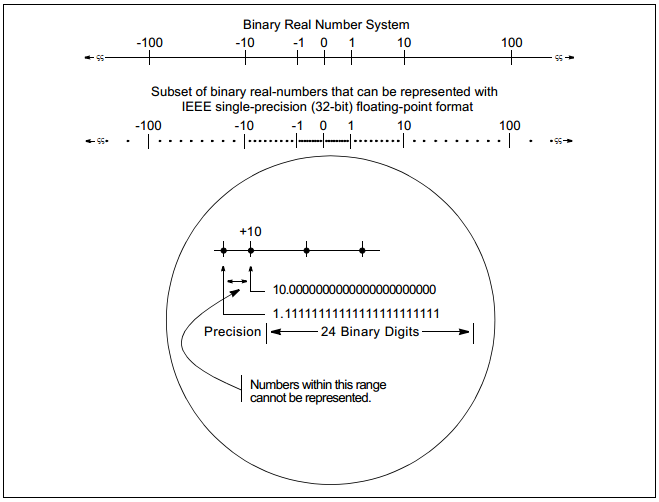
\includegraphics[scale=0.8]{MaNhiPhan.png}
				\end{center}
				\caption{Hệ thống mã nhị phân biểu diễn số thực}				
			\end{figure}
		\end{center}		
		
		Bởi vì kích thước và số lượng thanh ghi của bất kỳ máy tính nào có thể có hạn chế, chỉ có một đoạn mã nhị phân của số thực có thể được sử dụng trong tính toán số thực. Hình 3, phần số thực mà FPU hỗ trợ biểu diễn một giá trị xấp xỉ của một số thực. Phạm vi và độ chính xác của các phần mã nhị phân của số thực được biểu diễn theo định dạng FPU sử dụng để hiện thi cho số thực được sử dụng.
		
		\subsubsection*{Định dạng Floating-point}
		Để tăng tốc độ và hiệu quả của các phép tính số thực, các FPU hiện thị đại diện cho một số thực mà được biểu diễn theo định dạng floating-point. Trong định dạng này, một số thực có ba phần: bit dấu, định trị và số mũ. Định dạng này phù hợp với chuẩn IEEE.\\
		\begin{center}
			\begin{figure}[htp]
				\begin{center}
					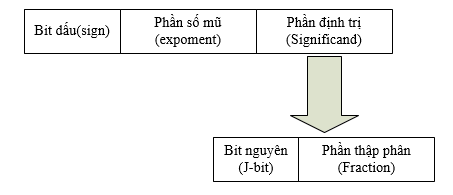
\includegraphics[scale=0.8]{DinhDangMNP.png}
				\end{center}
				\caption{Định dạng mã nhị phân của Floating-point}				
			\end{figure}
		\end{center}		
		
		Bit dấu là một giá trị nhị phân cho biết xem số đó là số âm (1) hay số dương (0). Phần định trị gồm hai phần: bit số nguyên (J-bit) và phần phân số. Phần bit số nguyên thường không được hiện thị, nhưng thay vào đó có giá trị mặc định. Phần số mũ là một số nguyên biểu diễn lũy thừa 2, điều này làm cho phần định trị được tăng lên.
		
		\subsubsection*{Số thông thường (normalized)}	
		Trong hầu hết mọi trường hợp, thanh ghi FPU hiển thị giá trị số thực định dạng thông thường. Ngoại trừ số 0 thì phần định trị luôn được tạo bởi một số thực và theo sau là phần phân số.
		\begin{itemize}
			\item[•	]1.fff…fff
		\end{itemize}
				
	\begin{longtable}{ | m{7cm} | m{7cm} | }
		\hline
				Ký hiệu & Giá trị\\
		\hline
		\hline
			Số thập phân	&178.125\\
		\hline	
			Số thập phân khoa học&	1.78124E102\\
		\hline	
			Số nhị phân khoa học	&1.0110010001E2111\\
		\hline	
			Số nhị phân khoa học (biểu diễn số mũ)	&1.0110010001E210000110\\
		\hline
			Đinh dạng số thực & 0(Bit dấu)  10000110(Phần mũ)	 011001000100000000000001(Phần định trị)\\
		\hline
	\end{longtable}		
		
		Đối với các giá trị thấp hơn 1 thì số 0 ở phia trước được loại bỏ (mỗi số 0 được loại bỏ, số mũ được tăng lên 1).\\

		Để hiện thị số lớn nhất của phần định trị theo định dạng thông thường thì phải cung cấp độ dài của phần định trị này. Để hiện thị số thực theo định dạng thông thường này thì phần định trị sẽ biểu diễn giá trị giữa 1 và 2, phần số mũ sẽ chỉ ra độ tăng của số thực đó.
		
		\subsubsection*{Số mũ (baised expoment)}
			Thanh ghi FPU biểu diễn số mũ theo định dạng cơ bản. Có nghĩa là một hằng số sẽ được thêm vào số mũ được biểu diễn vì vậy số mũ luôn là một số dương. Giá trị hằng số phụ thuộc vào số lượng bit được dùng để biểu diễn số thực trong định dạng dấu chấm phẩy động được sử dụng. Hằng số được chọn sao cho có thể thay đổi giá trị nhưng vẫn không bị tràn số.
			
			\subsubsection*{Số thực và mã hóa phi số thực}
			Có nhiều loại số thực và giá trị đặc biệt có thể được mã hóa theo định dạng dấu phẩy động của FPU:\\
			
			Những số đặc biệt và giá trị đặt biệt được chia thành các loại sau:
			\begin{itemize}
				\renewcommand{\labelitemi}{\textbullet}	
				\item Số 0.
				\item	Số hữu hạn không thông thường (denormalized).
				\item	Số hữu hạn thông thường (normalized).
				\item	Số vô cực
				\item	Không phải là một số (NaNs: Not a number )
				\item	Số không định nghĩa.
			\end{itemize}
			
			Hình ~\ref{fig:SothucNaN} sẽ chỉ rõ cách mã hóa số thực và phi số thực phù hợp với các biểu diễn số thực theo chuẩn IEEE. Ví dụ được sử dụng ở đây miêu tả chuẩn IEEE chính xác đơn (32-bit), các ký hiệu “S” chỉ bit dấu, “E” chỉ số mũ, “F” chỉ phần phân số. ( Giá trị của phần số mũ là một số nguyên). \\

		Các thanh ghi FPU có thể thực hiện các loại and/or trả về đúng giá trị, phụ thuộc vào phép toán được thực hiện. Các phần dưới đây sẽ mô tả các biểu diễn số thực và phi số thực.
		
		\subsubsection*{Số 0}
		Số 0 có thể được biểu diễn là +0 và  -0 phụ thuộc vào bit dấu. Việc mã hóa +0 và -0 tương đương nhau về mặt giá trị. Bít dấu của số 0 phụ thuộc vào phép toán được thực thi và cách thức làm tròn được sử dụng. Bit dấu số 0 có thể xác định tràn số dưới có đang xảy ra hay không, ngoài ra còn xác định bit dấu của giá trị vô cực. 
		
		\subsubsection*{Số normalized và denormalized}
		Trừ số 0, số thực được chia thành 2 dạng: normalized (bình thường) và denormalized (không bình thường). Số normalized bao gồm các giá trị khác 0, có thể mã hóa theo định dạng IEEE trong phạm vi từ số 0 đến vô cực. Trong hình 5, định dạng chính xác đơn với chỉ số mũ từ 0 đến 254 (phạm vi tham số -126 đến 126).
		\begin{center}
			\begin{figure}[htp]
				\begin{center}
					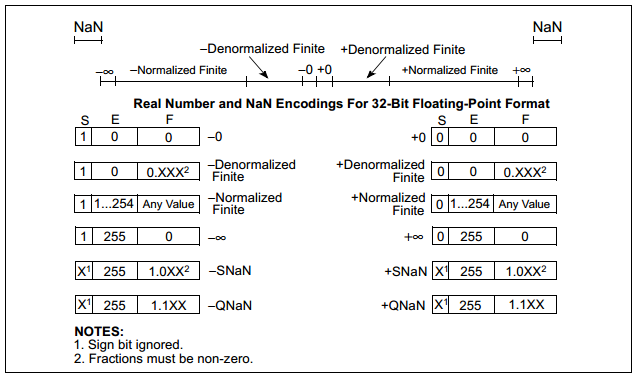
\includegraphics[scale=0.8]{SoThucNaN.png}
				\end{center}
				\caption{Số thực và NaN}				
				\label{fig:SothucNaN}
			\end{figure}
		\end{center}		

	Khi số thực càn gần về số 0, chiều dài bit dùng để biểu diễn số thực không đủ dài để biểu diễn. Bởi vì chỉ số mũ (trong ví dụ này là 32-bit) không đủ lớn để biểu diễn bit dịch phải để loại bỏ các bit 0 ở đầu (xem thêm phụ lục IEEE).\\

	Khi số mũ là số 0, những số nhỏ có thể được biểu diễn bằng những bit số nguyên (và những chuỗi bit ở đầu) của số 0. Số thực trong phạm vi này được gọi là denormalized (hay số rất nhỏ). Việc sử dụng các bit 0 ở đầu cho phép biểu diễn các số rất nhỏ nhưng những số rất nhỏ này là nguyên nhân mất đi sự chính xác (số bit trong phần định trị được giảm đi sẽ được tính toán dựa trên số bit 0 ở phần số mũ).\\

	Khi thực hiện các phép tính trên dấu chấm động, mỗi thanh ghi FPU thực hiện phép toán với số normalized và đưa ra kết quả là một số normalized. Số denormalized biểu diễn cho điều kiện tràn số dưới.\\
	
	Số denormalized được tính bằng kỹ thuật “gradual underflow”. Bảng () sẽ đưa ra một ví dụ của kỹ thuật “gradual underflow” trong xử lý tính toán số denormalized. Ở đây, sử dụng định dạng đơn nên số nhỏ nhất của số mũ là -126. Kết quả trong ví dụ này yêu cầu số mũ là -129. Nếu nhỏ hơn -129 là nằm ngoài phạm vi số mũ cho phép, kết quả của số denormalized bằng cách thêm các bit 0 ở đầu đến khi số mũ nhỏ nhất là -129.\\
		
		\begin{longtable}{ | m{4cm} | m{2cm} |  m{2cm} | m{4cm} | }
			\hline
				Toán hạng & Dấu & Số mũ* & Phần định trị\\
			\hline
			\hline
				Kết quả đúng & 0 & -129 & 1.01011100000..00\\
			\hline
				Số Denormalize & 0 & -128 & 0.10101110000..00\\
			\hline
				Số Denormalize & 0 & -127 & 0.01010111000..00\\
			\hline
				Số Denormalize & 0 & -126 & 0.00101011100..00\\
			\hline
				Kết quả Denormalize & 0 & -126 & 0.00101011100..00\\
			\hline
			\caption{Xử lý số denormalized}
		\end{longtable}
		
	
	Lưu ý: * Số mũ được biểu diễn trong phạm vi (-126 đến 126)\\

	Trong trường hợp tốt nhất, tất cả các bit của phần định trị được dịch phải bằng cách chèm thêm bit 0 ở đầu, tạo ra kết quả là số 0.\\

FPU xử lý với số demormal theo các cách sau đây: 
	\begin{itemize}
			\renewcommand{\labelitemi}{\textbullet}	
			\item	Không được phép tạo số denormalized.
			\item	Cung cấp xử lý ngoại lệ underflow để người lập trình có thể kiểm tra khi số denormalized được tạo ra.
			\item	Cung cấp các toán hạng xử lý số denormalized, cho phép chương trình kiểm tra khi mà các số denormalized được sử dụng như là một toán hạng. 
	\end{itemize}

	Khi một số denormalized ở định dạng chính xác đơn hoặc chính xác kép được sử dụng như một toán hạng, và xử lý ngoại lệ dernormal được đánh dấu, thanh ghi FPU sẽ tự động chuyển giá trị của số denormalized thành normalized bằng cách chuyển sang định dạng mở rộng.

		\subsubsection*{Số vô cực}
		Có 2 số vô cực là âm vô cực và dương vô cực được dùng để biểu diễn số thực âm nhỏ nhất và số thực dương lớn nhất vì vậy có thể biểu diễn dạng dấu chấm động. Số vô cực luôn được biểu diễn bằng bit 0 của phần định trị (phần phân số và bit số nguyên) và số mũ tối đa cho phép của mỗi định dạng (ví dụ: số mũ tối đa 255 đối với định dạng kép).\\

Bit dấu của số vô cực có thể dùng để so sánh. Số vô cực luôn được chỉ định rõ là âm vô cực luôn nhỏ hơn so với bất kỳ số thực cụ thể nào, dương vô cực luôn lớn hơn so với bất kỳ số thực cụ thể nào. Việc tính toán số vô cực luôn chính xác. Ngoại lệ được đánh dấu khi có phép toán xử dụng toán hạng là số vô cực, số vô cực được coi là toán hạng không hợp lệ. \\

Số denormalized biểu diễn cho điều kiện tràn số dưới, 2 số vô cực biểu diễn cho điều kiện tràn số trên. Kết quả số normlized của một phép toán có số mũ nằm trong phạm vi cho phép của số mũ phụ thuộc theo định dạng được sử dụng.
	
		\subsubsection*{NaNs (Not a number: không phải là một số)}
		NaN không phải là một, NaN là phần không nằm trên trục số thực trong hình 5. Việc mã hóa số NaN được chỉ ra trên trục số thực nằm ở cuối và đầu trục số. Khoảng trống này biểu diễn bất kỳ giá trị nào lớn với số mũ tối đa và phần phân số có bit khác không. (Bit dấu được bỏ qua đối với số NaN).\\

	Theo chuẩn IEEE có 2 định dạng cho NaN là: quiet NaNs(QNaNs) và signaling NaNs (SNaNs). Số QnaNs là NaN với phần phân số có hầu hết các bit là 1. Số SNaNs là NaN với phần phân số hầu hết các bit là 0. QNaNs cho phép tạo ra thông qua các phép toán mà không đánh dấu ngoại lệ nào. SNaNs thường thông báo một ngoại lệ không hợp lệ xảy ra khi thực hiện phép toán học. 
	
		\subsubsection*{Số không định nghĩa}
		Đối với mỗi loại dữ liệu của FPU, có một cách để mã hóa giá trị đặc biệt được gọi là giá trị không định nghĩa. Ví dụ, khi tính toán trên trường số thực, số không được định nghĩa là số QNaNs. FPU tạo ra giá trị không định nghĩa khi giá trị được đánh dấu xử lý ngoại lệ.
		
		\subsubsection{Kiến trúc FPU}
		Nhìn tổng quan kiến trúc, FPU là một bộ xử lý các thao tác hoạt động song song với bộ xử lý số nguyên. FPU có các câu lệnh cũng giống như các mã lệnh khác và được thực hiện tuần tự như bộ xử lý số nguyên và chia sẻ đường truyền với bộ xử lý số nguyên. Bộ xử lý FPU, bộ xử lý số nguyên hoạt động độc lập nhau và song song. 
		
		\begin{center}
			\begin{figure}[htp]
				\begin{center}
					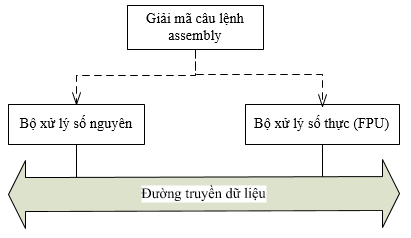
\includegraphics[scale=0.5]{FPUQuanHe.png}
				\end{center}
				\caption{Mối quan hệ giữa bộ xử lý FPU và bộ xử lý Integer}								
			\end{figure}
		\end{center}		
		
		Những câu lệnh được thực thi trong môi trường của FPU hình () bao gồm 8 thanh ghi dữ liệu (gọi là thanh ghi dữ liệu FPU) và sau đây là những thanh ghi với mục đích khác:
		\begin{itemize}
			\renewcommand{\labelitemi}{\textbullet}	
			\item	Thanh ghi trạng thái (the status register).
			\item	Thanh ghi điều khiển (the control register).
			\item	Thanh ghi thẻ (the tag word register).
			\item	Thanh ghi con trỏ lệnh (instruction poitnter register).
			\item	Thanh ghi toán hạng (last operand register).
			\item	Thanh ghi Opcode (Opcode register).
		\end{itemize}
		
	Những thanh ghi này được miêu tả trong phần tiếp theo.

		\subsubsection*{Thanh ghi dữ liệu FPU}
	Các thanh ghi dữ liệu FPU (hình 7 ) bao gồm 8 thanh ghi 80-bit. Giá trị được lưu trữ trong các thanh ghi theo định dạng mở rộng. Khi các số thực, số nguyên hoặc giá trị BCD được nén được nạp vào từ bộ nhớ vào trong thanh ghi dữ liệu FPU, các giá trị sẽ tự động chuyển về định dạng mở rộng. Khi tính toán, kết quả được chuyển lại vào bộ nhớ từ bất kỳ thanh ghi FPU, kết quả có thể đã được định dạng mở rộng hoặc được chuyển về định dạng FPU khác (số thực, số nguyên, giá trị BCD được nén).\\

	Những tập lệnh của FPU sẽ xử lý 8 thnh ghi dữ liệu nhưu là một ngăn xếp (stack) các thanh ghi (hình 7 ) tất cả địa chỉ ác thanh ghi dữ liệu là tương đối so với thanh ghi đỉnh của ngăn xếp. Số lượng thanh ghi ở đỉnh ngăn xếp hiện tại được lưu trữ trong trường TOP (stack TOP) trong thanh ghi trạng thái của FPU. Khi có 1 thao tác nạp thì TOP giảm đi 1 và nạp 1 giá trị vào thanh ghi ở đỉnh mới của ngăn xếp, và thao tác lưu trữ sẽ lưu trữ giá trị thanh ghi từ thanh ghi TOP hiện tại vào bộ nhớ.

		\subsubsection{Loại dữ liệu dấu chấm động và định dạng}
		\subsubsection{Câu lệnh FPU}	

\section{Windows API}

	\subsection{Một vài bộ thư viện cần hỗ trợ}

Ở những bước xây dựng đầu của đề tài, cần ưu tiên tiến hành cho những bộ thư viện phổ biến và được dùng rộng rãi trước tiên. Bảng 2 sau đây sẽ mô tả thông tin những bộ thư viện đã được hỗ trợ bởi BE-PUM:


\begin{longtable}{ | m{3cm} | m{11cm} | }
	\hline
Tên & Chức năng\\
	\hline
	\hline
Dịch vụ nền & Cho phép truy cập vào các nguồn tài nguyên cơ bản có sẵn trong hệ thống của Windows. Bao gồm những thứ như hệ thống tập tin, thiết bị, tiến trình (process), luồng (thread), xử lý lỗi (error handing).
Các chức năng này nằm trong tập tin kernel32.dll trên hệ điều hành Windows 32-bit.\\
	\hline
Dịch vụ nâng cao & Cho phép truy cập vào các chức năng bổ sung. Bao gồm những thứ như Windows registry, tắt/khởi động lại hệ thống (hoặc bãi bỏ - abort), bắt đầu/dừng/tạo ra một dịch vụ, quản lý tài khoản người dùng.
Các chức năng này nằm trong tập tin advapi32.dll trên hệ điều hành Windows 32-bit.\\
	\hline
Giao diện người dùng & Cung cấp các chức năng để tạo và quản lý cửa sổ màn hình và hầu hết những điều khiển cơ bản, chẳng hạn như nút và thanh cuộn, nhận chuột và bàn phím, cũng như các chức năng khác liên quan đến phần giao diện đồ họa người dùng của Windows.\\
	\hline
Các chức năng này nằm trong tập tin user32.dll trên hệ điều hành Windows 32-bit.
Windows shell & Cho phép các ứng dụng truy cập các chức năng được cung cấp bởi các shell của hệ điều hành, cũng như thay đổi nó.
Windows shell ở đây được hiểu là những thành phần cấu tạo nên giao diện đồ họa người dùng của hệ điều hành Windows (bao gồm những thứ như: màn hình desktop, thanh làm việc taskbar và các thành phần con trên nó,…).
Các chức năng này nằm trong tập tin shell32.dll trên hệ điều hành Windows 32-bit.\\
	\hline

\caption[Những bộ thư viện được hỗ trợ bởi BE-PUM]{Những bộ thư viện được hỗ trợ bởi BE-PUM}
\label{table:tblwapilib}
\end{longtable}


	\subsection{Trình tự các bước để ứng dụng JNA vào BE-PUM}

Để  tiến hành áp dụng những khả năng mang lại từ JNA và hệ thống BE-PUM, ta cần trải qua những bước sau đây:
\begin{enumerate}
	\item Ánh xạ tương ứng tên thư viện sẽ được gọi
	\item Ánh xạ tên hàm của API và những kiểu dữ liệu sẽ được dùng (bao gồm kiểu dữ liệu trả về và kiểu dữ liệu của các thông số đầu vào) từ ngôn ngữ lập trình C sang Java
	\item Tiến hành lấy giá trị bộ nhớ của các thông số đầu vào có trong BE-PUM
	\item Truyền các giá trị đó vào những kiểu tương ứng đã được ánh xạ trong Java, gọi API và lấy kết quả trả về.
	\item Lưu giá trị nhận được đó về lại bộ nhớ của BE-PUM
\end{enumerate}


	\subsection{Những kiểu dữ liệu và ánh xạ của chúng vào JNA}

Việc ánh xạ kiểu dữ liệu từ ngôn ngữ lập trình C sang Java được hỗ trợ sẵn bởi JNA cho một số kiểu cơ bản thường dùng như sau:\\

\begin{longtable}{ | m{3cm} | m{5cm} | m{5cm} | }
	\hline
STT & Kiểu dữ liệu trong C & Kiểu dữ liệu trong Java\\
	\hline
	\hline
1 & char & byte\\
	\hline
2 & wchar\_t & char\\
	\hline
3 & short & short\\
	\hline
4 & int & int\\
	\hline
5 & int & boolean\\
	\hline
6 & enum & int (thông thường)\\
	\hline
7  & long long, \_\_int64 & long\\
	\hline
8 & float & float\\
	\hline
9 & double & double\\
	\hline
10 & Con trỏ (VD: void*) & \specialcell{Buffer \\ Pointer}\\
	\hline
11 & \specialcell{Con trỏ (VD: void*, char*) \\ Mảng} & <P>[] (mảng của những kiểu nguyên thủy)\\
	\hline
12 & long & NativeLong\\
	\hline
13 & const char* & String\\
	\hline
14 & const wchar\_t* & WString\\
	\hline
15 & char** & String[]\\
	\hline
16 & wchar\_t** & WString[]\\
	\hline
17 & void** & Pointer[]\\
	\hline
18 & \specialcell{struct* \\ struct} & Structure\\
	\hline
19 & union & Union\\
	\hline
20 & struct[] & Structure[]\\
	\hline
21 & void (*FP)() & Callback\\
	\hline
22 & pointer (<T> *) & PointerType\\
	\hline

\caption[Một số ánh xạ kiểu dữ liệu cơ bản]{Một số ánh xạ kiểu dữ liệu cơ bản}
\label{table:tblwapi_type_mapping}
\end{longtable}
%\end{center}

Căn bản việc ánh xạ kiểu dữ liệu trong JNA được đáp ứng bằng việc kích thước dữ liệu được sử dụng giữa hai ngôn ngữ C và Java có kích thước bằng nhau. JNA hỗ trợ cho việc nạp một mảng các kí tự trong C bằng cách cho vào một đối tượng kiểu String.\\
 
Điểm hỗ trợ mạnh trong JNA đó là sử dụng và truy cập con trỏ của C thông qua đối tượng kiểu Pointer, dù rằng đang làm việc trong ngôn ngữ Java. Và nếu muốn lấy giá trị của một vùng nhớ thay vì chỉ một giá trị ô nhớ như Pointer, ta có thể sử dụng đối tượng kiểu Buffer để JNA đưa giá trị vùng nhớ đó vào trong đối tượng.


	\subsection{Dữ liệu kiểu cấu trúc (structure)} \label{sec:structure}

Một trong những lợi thế to lớn nhất mà JNA mang lại đó là nạp dữ liệu kiểu cấu trúc (structure) vào trong C mà ngôn ngữ Java không có. Điều này được hỗ trợ qua việc tạo ra một lớp mới, kế thừa từ lớp Structure của JNA.\\

Để tạo ra chính xác kiểu cấu trúc để nạp vào JNA, ta cũng phải tìm hiểu và nắm rõ các quy tắc xây dựng và làm việc với kiểu cấu trúc trong ngôn ngữ lập trình C.

		\begin{center}
			\begin{figure}[h]
				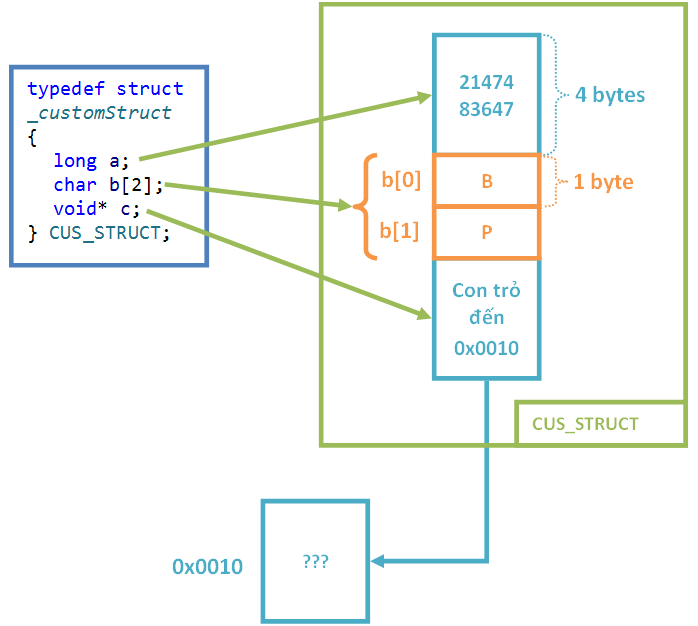
\includegraphics[scale=0.8]{StructureMemoryOrganization.png}
				\caption{Cách sắp xếp và lưu trữ bộ nhớ của structure}				
			\end{figure}
		\end{center}

Một struct trong ngôn ngữ lập trình C là một khai báo dữ liệu kiểu phức hợp, trong đó nó định nghĩa một danh sách các biến được đặt bên trong một khối bộ nhớ. Nó cho phép các biến khác nhau được truy xuất thông qua một con trỏ duy nhất (con trỏ của structure). Một structure có khả năng chứa nhiều kiểu dữ liệu khác nhau từ kiểu dữ liệu nguyên thủy đến kiểu dữ liệu phức tạp khác (enum, structure).\\

Định nghĩa struct khá giống với định nghĩa lớp trong Java, nhưng struct không hề có khả năng khai báo phương thức, cũng như các từ khóa public, private,… như Java. Thêm vào đó, cơ chế cấp phát bộ nhớ của struct chỉ đơn thuần là sự sắp xếp liên tục của các vùng nhớ chứa giá trị của các biến đã được khai báo bên trong. Cách sắp xếp này hoàn toàn tương ứng với ngôn ngữ assembly; do đó ta cần đảm bảo việc lấy ra và gán trở lại bộ nhớ BE-PUM một cách chính xác theo trình tự như vậy.



\chapter{Thiết Kế Và Xây Dựng}
\section{Các câu lệnh hợp ngữ}
	\subsection{Sơ đồ chương trình BE-PUM}
		BE-PUM được xây dựng chủ yếu trên mã nguồn của JakStab do đó hình ~\ref{fig:SoDoClass} thể hiện phần BE-PUM đang được phát triền. Dưới dây là sơ đồ class chương trình:
		\begin{center}
			\begin{figure}[htp]
				\begin{center}
					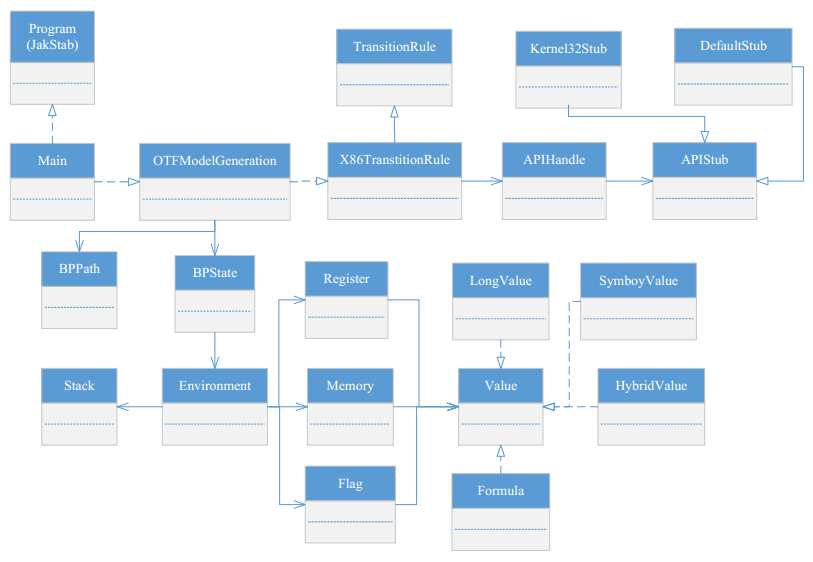
\includegraphics[scale=0.5]{SoDoClass.png}
				\end{center}
				\caption{Sơ đồ class chương trình BE-PUM}	
					\label{fig:SoDoClass}		
			\end{figure}
		\end{center}			
			
		Sơ đồ thể hiện mối liên hệ giữa các class với nhau. Trong sơ đồ không thể hiện các biến của class, các hàm của class, mục đích của sơ đồ thể hiện mối liên kết giữa các class với nhau. Class \textit{Program} là một class được phát triển từ dự án JakStab, BE-PUM kế thừa và phát triền lên. Class chính của BE-PUM là class \textit{Main}, nơi gọi chương trình cần phân tích. Class \textit{Main} sẽ gọi class \textit{OTFModelGeneration} để tạo ra sơ đồ CFG(control flow graph: sơ đồ điều khiển) với mỗi đỉnh là một câu lệnh assembly được dịch từ mã nhị phân của chương trình cần phân tích. Mỗi câu lệnh assembly có các biến môi trường khác nhau. Class \textit{Environment} có nhiệm vụ thể hiện môi trường làm việc của từng câu lệnh. Biến môi trường có các thành phần khác nhau như \textit{Register, Flag, Stack, Memory}cũng được hiện thực bằng các class tương ứng.\\
		
		Class  \textit{X86TransitionRule} có nhiệm vụ hiện thực mô phỏng các câu lệnh assembly. Để hiện thực mô phỏng các câu lệnh khác nhau, class \textit{X86TranstitionRule} được hỗ trợ thêm các class khác sẽ được trình bày trong phần "phân tích class mô phỏng câu lệnh Assembly". Class\textit{X86TranstitionRule} cũng đảm nhiệm việc tiến hành phân tích từng câu lệnh assembly, trong quá trình phân tích sẽ  co API (Microsoft Windows application programming interface) tham gia, vấn đề về API sẽ được đề cập đến phần "Window API".
		
	\subsection{Phân tích class mô phỏng câu lệnh Assembly}
	Hình ~\ref{fig:SoDoClassAss}	mô tả lược đồ lớp (class)  chính dùng đề mô phỏng câu lệnh assembly. Class quan trong \textit{X86TransitionRule} và\textit{Simulation Assembly} dùng để mô phỏng thao tác thực hiện của các câu lệnh assembly. Ngoài ra còn có class Environment mô phỏng các biến sẽ bị thay đổi khi câu lệnh assembly được thực thi. Các class \textit{FPUStatusWord, FPURegister, FPUControlWord} mô phỏng lại các biến môi trường mà các câu lệnh assembly xử lý FPU (Floatting-Point Unit) sử dụng. Class \textit{Register, Flag, Stack, Memory} mô phỏng lại các câu lệnh assembly thao tác trên số nguyên.
	
	Trong phần này sẽ phân tích môi trường cần để câu lệnh assembly xử lý số nguyên thực hiện và môi trường FPU xử lý số thực. Câu lệnh xử lý số nguyên và số thực tuy cùng mục đích thực hiện nhưng khi thao tác và thực hiện câu lệnh, các biến môi trường được sử dụng khác nhau. Nên việc thao tác, phân tách các biến môi trường sao cho phù hợp với hai nhóm xử lý số nguyên.
	
		\begin{center}
			\begin{figure}[htp]
				\begin{center}
					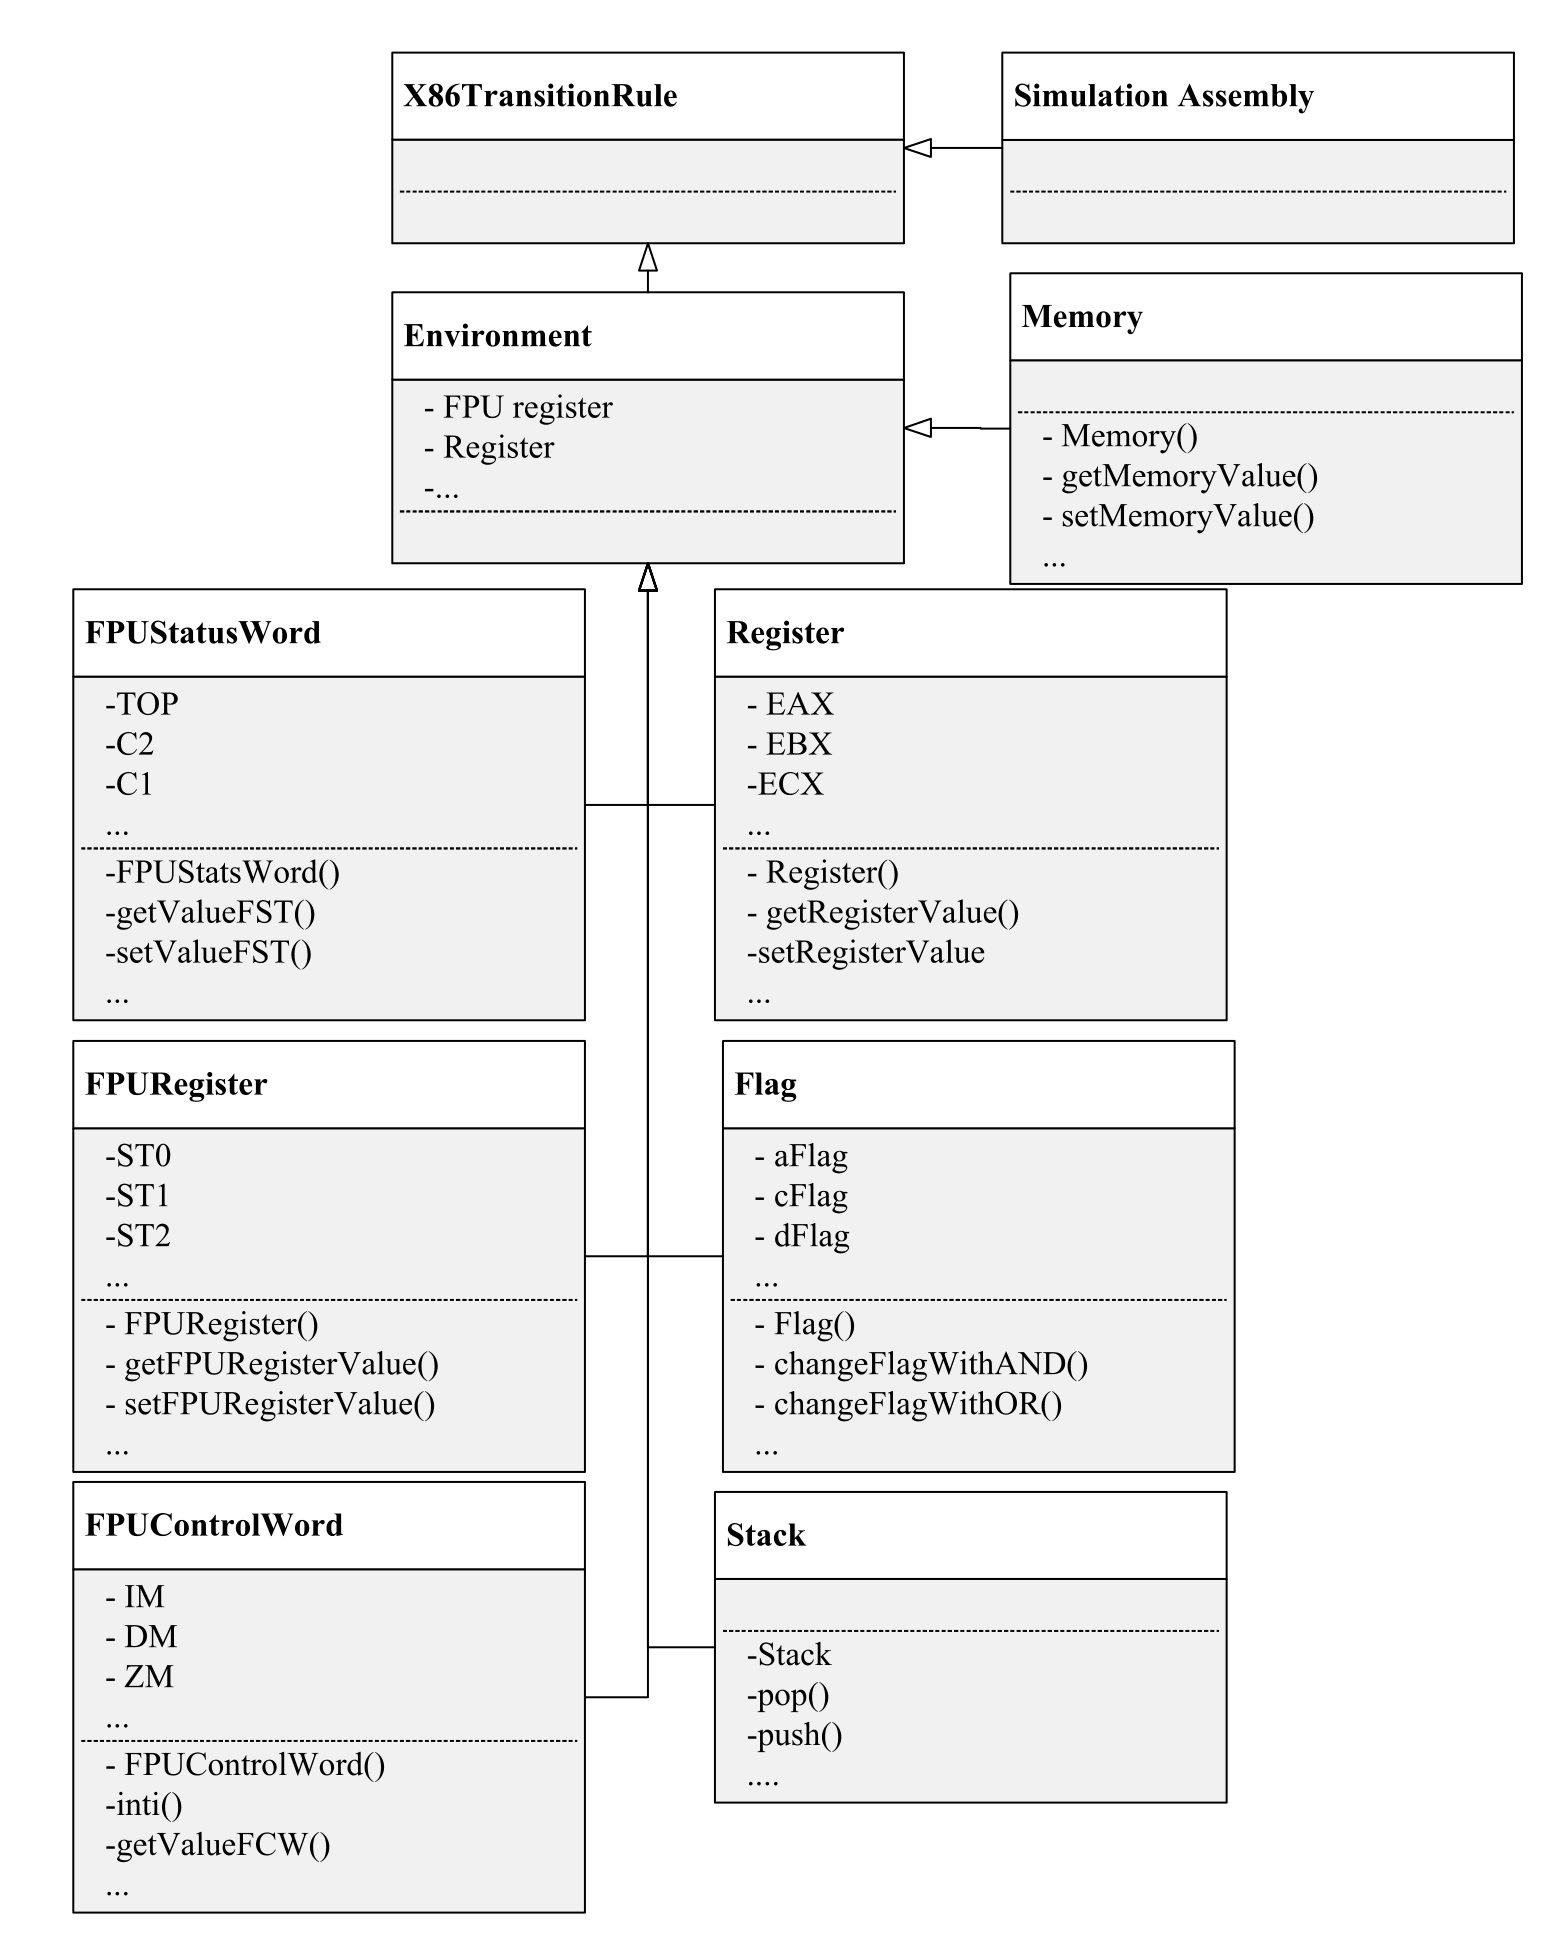
\includegraphics[scale=0.4]{UMLAss.png}
				\end{center}
				\caption{Sơ đồ class mô phỏng câu lệnh Assembly}	
					\label{fig:SoDoClassAss}		
			\end{figure}
		\end{center}			
		
		Để thể hiện các biến môi trường các class Register, Flag, Stack, FPUStatusWord, FPURegister, FPUControlWord,  Be-Pum xây dựng các class Environment để hỗ trợ trong việc truy xuất, thao tác.
	
		\begin{center}
			\begin{figure}[htp]
				\begin{center}
					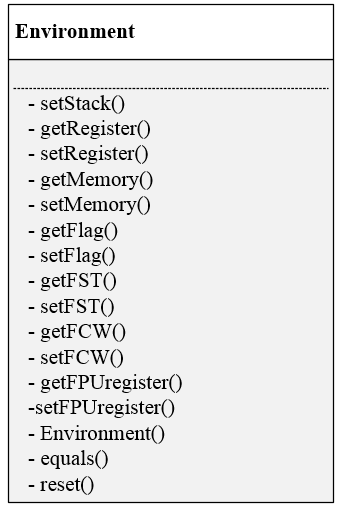
\includegraphics[scale=0.75]{ClassEnv.png}
				\end{center}
				\caption{Class Environment}	
					\label{fig:ClassEnv}		
			\end{figure}
		\end{center}					
		
		Class Environmet có nhiệm vụ liên kết các class Stack, Register, Memory, Flag, FPUStatusWord, FPURegister, FPUControlWord, để thao tác truy xuất trực tiếp lên các biến môi trường này. Class Enviroment hiện thực các hàm để hỗ trợ thao tác truy xuất thuận tiện hơn. Ngoài ra, hiện thực hàm equals() để so sánh biến môi trường của câu lệnh assembly này với biến môi trường của câu lệnh assembly khác. Từ đó hỗ trợ trong việc đánh giá, phân tích câu lệnh assembly.
		
		\newpage
	\subsection*{Môi trường xử lý số nguyên}
	Class Environmet liên kết với class Stack, hình () thể hiện class Stack.
		\begin{center}
			\begin{figure}[htp]
				\begin{center}
					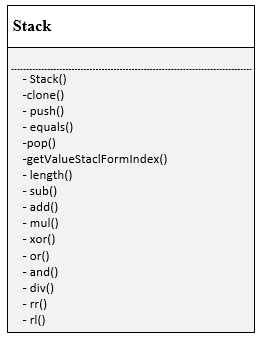
\includegraphics[scale=1.0]{ClassStack.png}
				\end{center}
				\caption{Class Stack}	
					\label{fig:ClassStack}		
			\end{figure}
		\end{center}		
	
	Class Stack gồm các hàm hỗ trợ thao tác trên stack của chương trinh. Hàm push() và pop() là hai hàm quan trọng có nhiệm vụ thao tác cơ bản trên stack là đưa vào ngăn xếp và lấy ngăn xếp ra. Ngoài ra còn có các hàm length() thể hiện kích thước stack, equals() để so sánh hai stack với nhau, việc này hỗ trợ rất nhiều trong qua trình phân tích hay so trùng được sử dụng trong các kỹ thuật phân tích virus. Ngoài ra còn có các hàm để hỗ trợ thao tác toán học như add() để cộng thêm một số, sub() để nhân với một số,…
	
	\newpage
	Class Register được hiện thực như các thanh ghi Register trong hợp ngữ assembly. Hình () thể hiện class Register:
	\begin{center}
			\begin{figure}[htp]
				\begin{center}
					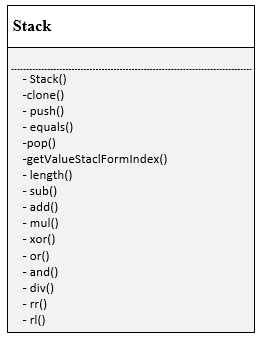
\includegraphics[scale=1.0]{ClassStack.png}
				\end{center}
				\caption{Class Stack}	
					\label{fig:ClassStack}		
			\end{figure}
		\end{center}		
		
		Class Register gồm các biến được thể hiện là các thanh ghi Register được sử dụng trong hợp ngữ assembly. Các biến này sẽ lưu giá trị của thanh ghi trong quá trình thực thi chương trình cần phân tích. Mỗi giá trị của biến có thể bị thay đổi khi thực hiện phân tích từng câu lệnh assembly của chương trình cần phân tích. Class Resgister xây dựng các hàm hỗ trợ thao tác trên thanh ghi như getRegiterValue() có nhiệm vụ lấy giá trị của thanh ghi nào đó, setRegisterValue() có nhiệm vụ gán lại giá trị của một thanh ghi. Ngoài ra, class Register còn hiện thực một số hàm hỗ trợ thao tác toán học trên thanh ghi như: add() có nhiệm vụ cộng thêm một giá trị nào đó vào thanh ghi, and() có nhiệm vụ như thực hiện phép and (đại số Boole),.. những hàm này giúp hỗ trợ nhanh trong việc hiện thực câu lệnh sau này.
		
		\newpage
		Class Register được hiện thực như các thanh ghi Register trong hợp ngữ assembly. Hình () thể hiện class Register:
		\begin{center}
			\begin{figure}[htp]
				\begin{center}
					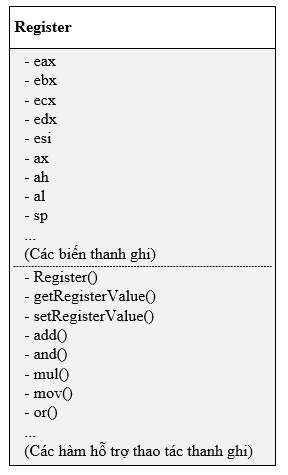
\includegraphics[scale=1.0]{ClassRegister.png}
				\end{center}
				\caption{Class Register}	
					\label{fig:ClassRegister}		
			\end{figure}
		\end{center}		
			
	Class Register gồm các biến được thể hiện là các thanh ghi Register được sử dụng trong hợp ngữ assembly. Các biến này sẽ lưu giá trị của thanh ghi trong quá trình thực thi chương trình cần phân tích. Mỗi giá trị của biến có thể bị thay đổi khi thực hiện phân tích từng câu lệnh assembly của chương trình cần phân tích. Class Resgister xây dựng các hàm hỗ trợ thao tác trên thanh ghi như getRegiterValue() có nhiệm vụ lấy giá trị của thanh ghi nào đó, setRegisterValue() có nhiệm vụ gán lại giá trị của một thanh ghi. Ngoài ra, class Register còn hiện thực một số hàm hỗ trợ thao tác toán học trên thanh ghi như: add() có nhiệm vụ cộng thêm một giá trị nào đó vào thanh ghi, and() có nhiệm vụ như thực hiện phép and (đại số Boole),.. những hàm này giúp hỗ trợ nhanh trong việc hiện thực câu lệnh sau này.
	
		\newpage
	Class Memory được hiện thực như là các thao tác trên một bộ nhớ được sử dụng trong hợp ngữ assembly. Hình () thể hiện class Memory: 
	
		\begin{center}
			\begin{figure}[htp]
				\begin{center}
					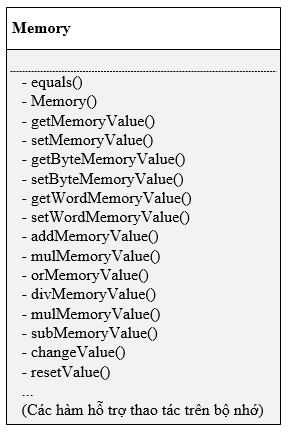
\includegraphics[scale=1.0]{ClassMemory.png}
				\end{center}
				\caption{Class Memory}	
					\label{fig:ClassMemory}		
			\end{figure}
		\end{center}		
	
	Class Memory gồm các hàm được hiện thực để hỗ trợ trong việc thao tác với địa chỉ bộ nhớ. Mỗi hàm được hiện thực có nhiệm vụ khác nhau nhưng cùng một mục đích là phân tích câu lệnh assembly như hàm equals() dùng để so sánh bộ nhớ, getMemoryValue() dùng để lấy giá trị của địa chỉ bộ nhớ đó, setMemoryValue() dùng để gán lại giá trị của bộ nhớ, getByteMemoryValue() dùng để lấy giá trị Byte của địa chỉ bộ nhớ, ngoài ra còn có các hàm hỗ trợ thao tác toán học được sử dụng trên bộ nhớ như hàm addMemoryValue() dùng để cộng thêm một số vào giá trị bộ nhớ, mulMemoryValue() dùng để nhân thêm một số vào giá trị bộ nhớ, changeValue() với địa chỉ xác định dùng để thay đổi giá trị của địa chỉ bộ nhớ đó, việc thay đổi giá trị tại địa chỉ bộ nhớ giúp hỗ trợ trong quá trình phân tích, đọc hiểu mã assembly.
	
	\newpage
	Class Flag được hiện thực như các Flag trong hợp ngữ assembly. Hình () thể hiện class Flag của chương trình BE-PUM:	
		\begin{center}
			\begin{figure}[htp]
				\begin{center}
					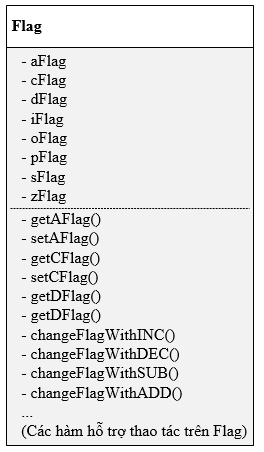
\includegraphics[scale=1.0]{ClassFlag.png}
				\end{center}
				\caption{Class Flag}	
					\label{fig:ClassFlag}		
			\end{figure}
		\end{center}			
	
Class Flag gồm các biến được phỏng theo các biến Flag được sử dụng trong hợp ngữ assembly, mỗi tên biến tương với mỗi giá trị Flag trong quá trình phân tích. Các giá trị của Flag sẽ thay đổi theo từng câu lệnh assembly, dựa vào xự thay đổi này để hỗ trợ trong quá trình phân tích chương trình. Ngoài ra, class Flag còn hiện thực thêm một số hàm để hỗ trợ trong quá trình phân tích như getAFlag() để lấy giá trị của aFlag, setAFlag() để thay đổi giá trị của aFlag, tương tự như vậy đối với các biến đã được mô phỏng. Thêm vào đó là các hàm thay đổi Flag theo các câu lệnh hỗ trợ toán học như hàm changeFlagWithINC() có nhiệm vụ thay đổi các giá trị của Flag tương ứng khi thực hiện câu lệnh INC (tăng giá trị), changeFlagWithSUB() thay đổi Flag khi thực hiện phép toán công (SUB),… Tương tự như vậy, class tiếp tục xây dựng các hàm hỗ trợ thay đổi nhanh khi thực hiện các phép toán.


	\newpage
	Class X86TranstitionRule là class đặc biệt quan trọng, là nơi xử lý các câu lệnh assembly, class X86TranstitionRule được hỗ trợ bởi nhiểu class con khác để thực hiện việc phân tích mã assembly. Hình () biểu diễn class X86TranstitionRule:
	\begin{center}
			\begin{figure}[htp]
				\begin{center}
					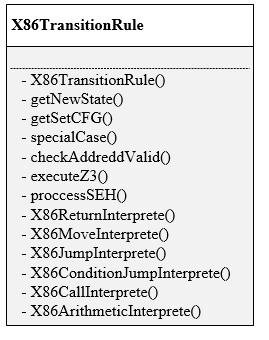
\includegraphics[scale=1.0]{ClassTransitionRule.png}
				\end{center}
				\caption{Class X86TransitionRule	}	
					\label{fig:ClassFlag}		
			\end{figure}
		\end{center}			
		
	Class X86TransitionRule được hiện thực các hàm để hỗ trợ trong quá trình phân tích chương trình assembly. Mỗi đỉnh trong đồ thị phân tích là một câu lệnh, mỗi câu lệnh có nhiệm vụ, chức năng khác nhau. Do đó, cần phần nhóm các câu lệnh để hiện thực. Trong class X86TransitionRule, các hàm được chia theo nhóm câu lệnh như X86IntrustionInterprete() hiện thực các câu lệnh cơ bản thường dùng như STD (gán giá trị dFlag = 1) cmovcc (các điều kiện gán)… X86RetrunInterprete() hiện thực các câu lệnh trả kết quả về như RET (kết quả trả về khi kết thúc một hàm), X86MoveInterprete() hiện thực các câu liên quan đến gán giá trị như MOV, MOVZ,… tương tự như vậy các nhóm câu lệnh nhảy, biểu thức toán học, các câu lệnh gọi hàm được hiện thực. Ngoài ra còn có các hàm hỗ trợ trong việc phân tích và tính toán như hàm executeZ3() có nhiệm vụ gọi thư viện Z3 để tính toán. Đây làm class rất quan trọng vì class này đảm nhận nhiệm vụ phân tích chương trinh assmebly từ đó đưa ra kết quả.
	
	\subsection*{Môi trường xử lý số thực}
	

		
\newpage
\section{Windows API} \label{sec:wapi_design}

	\subsection{Các thành phần chính của bộ xử lý Windows API} \label{sec:main_classes}

	\begin{figure}[htp]
	\centering
		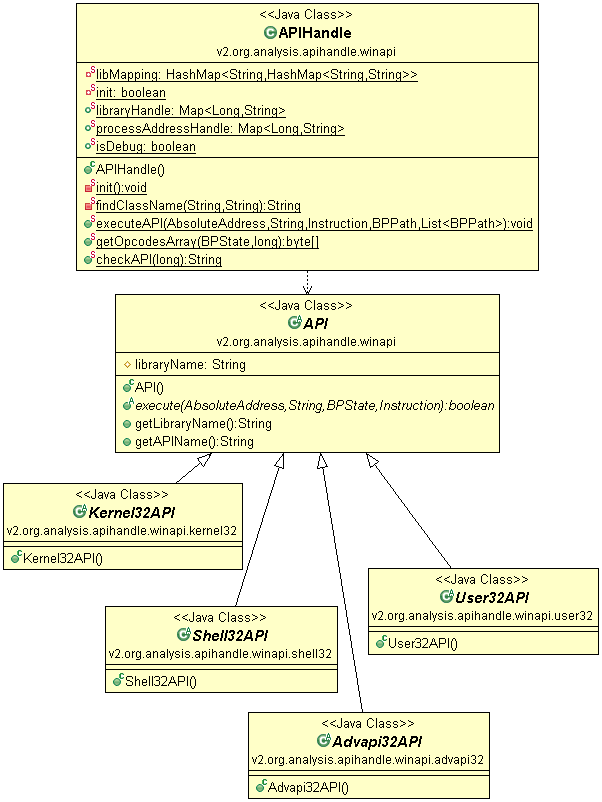
\includegraphics[scale=0.74]{wapi_1_main_classes.png}
		\caption{Kiến trúc chính của bộ xử lý Windows API dành cho BE-PUM}	
		\label{fig:wapi_1_main_classes}		
	\end{figure}

Hình \ref{fig:wapi_1_main_classes} mô tả lược đồ lớp (class) chính được xây dựng cho bộ xử lý Windows API. Trong đó có một class nắm giữ toàn bộ giao tiếp và làm việc giữa hệ thống BE-PUM và các xử lý chính cho từng API đó là class \textit{APIHandle}. Mỗi khi hệ thống BE-PUM cần xử lý một API bất kỳ nào đó, phương thức \textit{executeAPI} của \textit{APIHandle} sẽ được gọi để làm việc.\\

Kiến trúc chính của đề tài được xây dựng dựa trên dạng thức thiết kế adapter hay còn gọi là dạng thiết kế điều hợp. Với adapter là lớp trừu tượng – abstract class: lớp \textit{API}, mỗi bộ thư viện Windows API sẽ được trừu tượng hóa thành từng abstract class mà sẽ kế thừa từ lớp \textit{API} (ví dụ như các lớp \textit{Kernel32API}, \textit{User32API},…). Rồi sau đó, mỗi Windows API sẽ được trừu tượng hóa thành một class, được đặt tên trùng với tên của chính Windows API đó, kèm theo sẽ là việc kế thừa và hiện thực đúng abstract class của bộ thư viện mà Windows API thuộc về.\\

Hình \ref{fig:wapi_2_implemented_classes} ngay sau đây sẽ mô tả ngắn gọn cho việc hiện thực từng Windows API của bộ thư viện dịch vụ nền được chứa trong tập tin \textit{kernel32.dll}.

	\begin{figure}[htp]
	\centering
		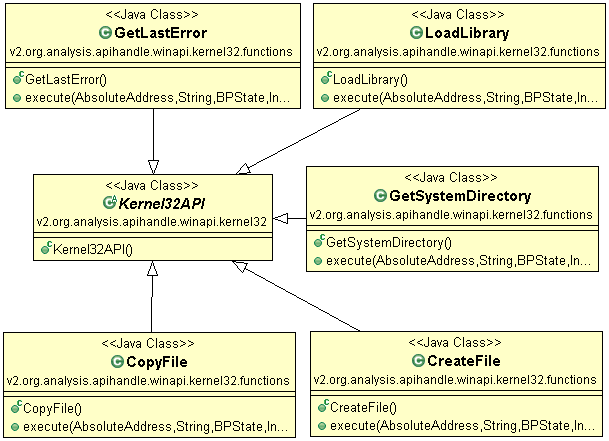
\includegraphics[scale=0.74]{wapi_2_implemented_classes}
		\caption{Mô hình hiện thực một số Windows API trong \textit{kernel32.dll}}	
		\label{fig:wapi_2_implemented_classes}		
	\end{figure}

	\newpage
	\subsection{Những khai báo ánh xạ của bộ xử lý Windows API} \label{sec:mapping}

Ngoài những thành phần chính nêu trên, bộ xử lý Windows API còn có những lớp khác để nắm thông tin ánh xạ giữa hai ngôn ngữ lập trình Java và C thông qua JNA.

	\begin{figure}[H]
	\centering
		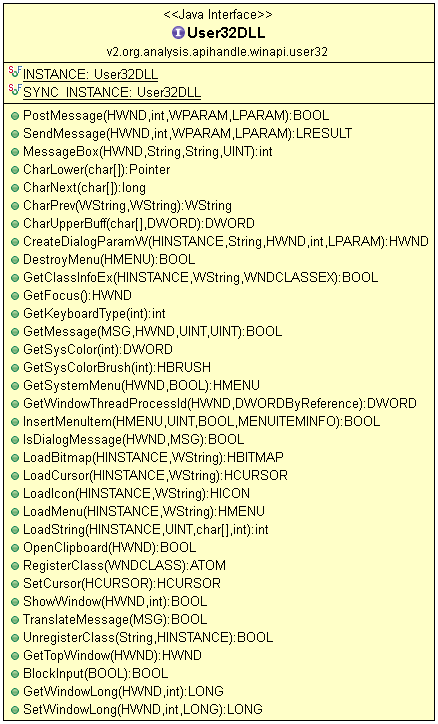
\includegraphics[scale=0.74]{wapi_3_function_map.png}
		\caption{Lớp chứa thông tin ánh xạ những Windows API trong \textit{user32.dll}}	
		\label{fig:wapi_3_function_map}		
	\end{figure}

Trong Hình \ref{fig:wapi_3_function_map} là một mô tả về ánh xạ tên hàm và kiểu dữ liệu đầu vào của bộ thư viện giao diện người dùng được chứa trong tập tin \textit{user32.dll}. Ngoài ra, bộ thư viện JNA có khai báo ánh xạ sẵn một số hàm Windows API cùng những kiểu dữ liệu chính mà Windows API thường dùng, nhờ đó mà những kiểu dữ liệu thông dụng như \textit{HWND, HINSTANCE, LPARAM, DWORD,…} không đòi hỏi lập trình viên phải khai báo và ánh xạ lại.\\

Nhưng không phải tất cả kiểu dữ liệu đề có sẵn, đặc biệt là những kiểu dữ liệu cấu trúc, cần có những trường hợp phải khai báo thêm để ánh xạ và phục vụ cho đề tài này.

	\begin{figure}[H]
	\centering
		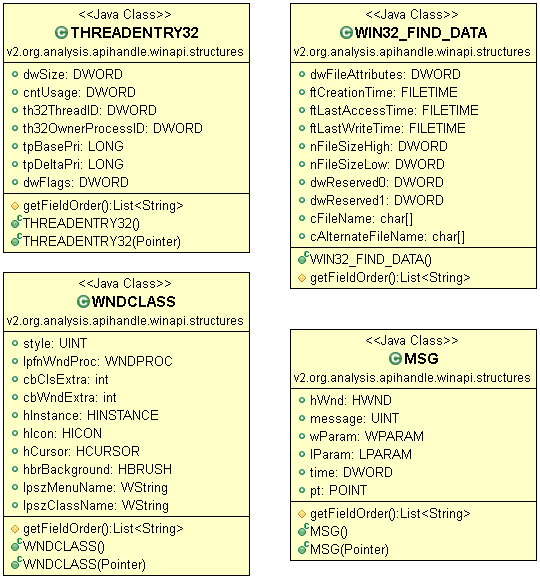
\includegraphics[scale=0.74]{wapi_4_structure}
		\caption{Một số dữ liệu kiểu cấu trúc được xây dựng thêm}	
		\label{fig:wapi_4_structure}		
	\end{figure}

Nội dung của Hình \ref{fig:wapi_4_structure} thể hiện khai báo thêm của một số dữ liệu kiểu cấu trúc dành cho đề tài này. Như đã nói ở Mục \ref{sec:structure}, việc xây dựng này đòi hỏi phải chính xác về kích thước và trình tự các biến được khai báo bên trong struct, để dữ liệu được nạp ra vào chính xác.

	\subsection{Kiến trúc xây dựng và làm việc}

Từ những thành phần đã trình bày ở Mục \ref{sec:main_classes} và Mục \ref{sec:mapping}, kiến trúc của bộ xử lý Windows API sẽ được tổ chức lại cho thống nhất và dễ dàng mở rộng về sau:

	\begin{figure}[H]
	\centering
		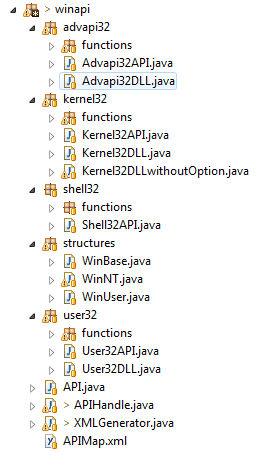
\includegraphics[scale=0.74]{wapi_5_tree}
		\caption{Cây cấu trúc mô tả những thành phần trong bộ xử lý Windows API}	
		\label{fig:wapi_5_tree}		
	\end{figure}

Gói ngoài cùng của bộ xử lý \textit{(winapi)} sẽ nắm:

\begin{itemize}
	\item Khai báo lớp trừu tượng \textit{API}: đặc tả phương thức thực thi dùng chung cho mọi Windows API;

	\item Lớp \textit{APIHandle}: giao tiếp chính giữa bộ xử lý Windows API và hệ thống BE-PUM;

	\item Những gói được đặt tên ứng với từng tên tập tin (không bao gồm phần mở rộng) mà bộ thư viện đó thuộc về. Mỗi gói đó sẽ chứa những thành phần như sau:

	\begin{itemize}
		\item Lớp khai báo trừu tượng cho từng Windows API của bộ thư viện đó (ví dụ như lớp \textit{Kernel32API}), trong đó sẽ nạp vào tên của bộ thư viện hiện tại;

		\item Lớp khai báo ánh xạ thư viện và tên hàm mà hiện bộ thư viện JNA chưa có sẵn (chỉ tồn tại trong trường hợp những Windows API mà đề tài hiện thực chưa có trong bộ thư viện JNA)

		\item Một gói được đặt tên \textit{functions}: dùng để chứa mọi lớp xử lý cho từng Windows API của bộ thư viện hiện tại (ví dụ như hiện tại gói bên ngoài là \textit{kernel32}, những hàm Windows API được xây dựng bên trong sẽ là: \textit{CreateFile, CopyFile, GetLastError…}).
	\end{itemize}

	\item Gói \textit{structures}: chứa những lớp khai báo ánh xạ dữ liệu kiểu cấu trúc mà bộ thư viện JNA chưa có sẵn.

	\item Lớp \textit{XMLGenerator}: có chức năng sinh ra tự động tập tin cấu trúc XML từ tổ chức như trên của bộ xử lý Windows API, mô tả ánh xạ giữa tên của hàm Windows API và tên đầy đủ của lớp sẽ đảm nhận việc xử lý hàm Windows API đó, kèm theo là nó thuộc tập tin thư viện nào. Ví dụ như sau:\\


\lstset{language=HTML}
\begin{lstlisting}
<APIMap>
	<DLL name="advapi32">
		<API funcName="cryptdecrypt" 
className="advapi32.functions.CryptDecrypt"/>
	</DLL>
	<DLL name="kernel32">
		<API funcName="closehandle" 
className="winapi.kernel32.functions.CloseHandle"/>
	</DLL>
</APIMap>
\end{lstlisting}

	\item Tập tin \textit{APIMap.xml}: là nội dung do lớp \textit{XMLGenerator} sinh ra.
\end{itemize}

Nội dung của tập tin \textit{APIMap.xml} được sinh ra dùng để làm chỉ mục cho lớp trung gian \textit{APIHandle} biết được rằng: với thông tin đầu vào là tên của Windows API mà hệ thống BE-PUM yêu cầu, thì lớp nào sẽ xử lý được yêu cầu đó. Sau khi có được tên đầy đủ của lớp xử lý, \textit{APIHandle} sẽ khởi tạo lớp đó với kiểu đối tượng là \textit{API} (do tất cả lớp xử lý đều hiện thực trên lớp này), rồi sau đó gọi phương thức \textit{execute} để đối tượng này xử lý toàn bộ.

	\begin{figure}[H]
	\centering
		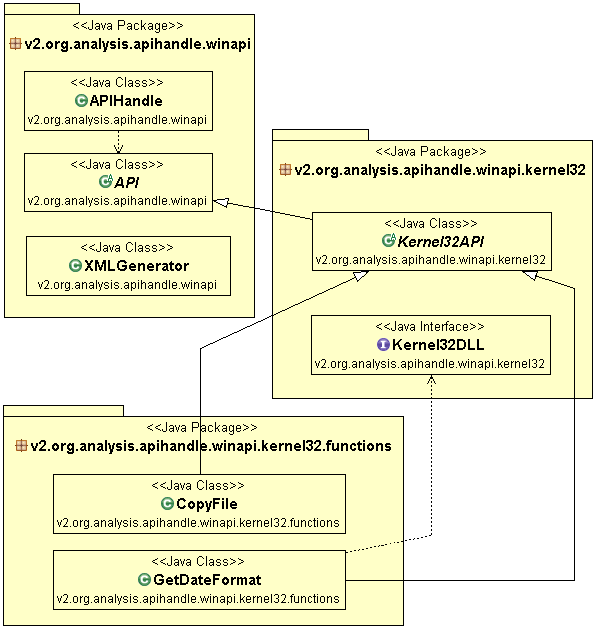
\includegraphics[scale=0.74]{wapi_6_inherited}
		\caption{Giản đồ thể hiện mối liên hệ giữa các thành phần}	
		\label{fig:wapi_6_inherited}		
	\end{figure}


Với việc tổ chức theo cấu trúc này và sinh ra tập tin đánh chỉ mục thì sẽ có được những ưu điểm sau đây:

\begin{itemize}
	\item Dễ dàng quản lý mã nguồn: do Windows API có rất rất nhiều hàm, việc tạo ra mỗi lớp độc lập để xử lý cho từng hàm Windows API sẽ giúp cho mã nguồn được rõ ràng và độc lập cũng như việc sửa chữa sau này được tiện lợi;

	\item Dễ dàng bổ sung: nếu muốn hiện thực thêm một Windows API bất kỳ, ta chỉ việc tạo ra một lớp theo đúng quy định cấu trúc như trên, lớp XMLGenerator sẽ giúp sinh ra nội dung của tập tin APIMap.xml và chỉ đơn giản như vậy là đã tích hợp được một Windows API mới.
\end{itemize}

Nội dung của Hình \ref{fig:wapi_6_inherited} trình bày ví dụ về mối liên hệ mà cấu trúc vừa nêu. Khi hệ thống BE-PUM yêu cầu lớp APIHandle xử lý hàm CopyFile, nó sẽ dùng APIMap.xml để tìm được tên đầy đủ của lớp xử lý được hàm này. Tên ấy được dùng để khai báo khởi tạo động một đối tượng bất kỳ và sau đó ép kiểu về kiểu đối tượng API. Do lớp xử lý được hàm này được hiện thực dựa trên lớp trừu tượng API. Còn với trường hợp nếu là hàm GetDateFormat, thì trong lớp này còn có sử dụng lớp Kernel32DLL do bộ thư viện JNA chưa khai báo sẵn hàm này.

	\subsection{Quản lý môi trường tương tác vật lý}

Do một số Windows API có khả năng làm việc với hệ thống tập tin lưu trữ, dẫn đến khả năng làm ảnh hưởng xấu đến hệ thống do chúng ta đang tập trung vào việc phân tích những phần mềm độc hại cho máy vi tính. Vì vậy ta cần quản lý và ngăn chặn việc đó.\\

Để hiện thực việc đó, một lớp mang tên \textit{Storage} được viết ra để ánh xạ toàn bộ địa chỉ của hệ thống thật vào một vùng lưu trữ đã được quy định. Và rồi mỗi khi một Windows API nào có sử dụng đường dẫn để làm việc, thì cần phải kiểm tra rằng liệu Windows API đó có khả năng ảnh hưởng đến hệ thống hay không, nếu có ta cần ánh xạ sang vùng lưu trữ đã được quản lý để tránh những nguy hại.


\chapter{Kết Quả}
\section{Thí nghiệm và đánh giá kết quả}

\section{Các câu lệnh hợp ngữ đã được hỗ trợ}

\section{Các Windows API đã được hỗ trợ}

\chapter{Hướng Phát Triển Trong Tương Lai}
\section{Tăng số lượng các câu lệnh hợp ngữ được hỗ trợ}

\section{Tăng số lượng các Windows API được hỗ trợ}

Ở thời điểm hiện tại, số lượng các Windows API đã được hỗ trợ cho BE-PUM vẫn còn rất ít ỏi. Bởi thực tế, con số Windows API mà hệ điều hành Windows đang cung cấp vượt xa con số đó. Theo một thống kê nhỏ từ những bộ thư viện thường dùng của Windows, số lượng Windows API hiện đang được cung cấp lên đến khoảng 4000 hàm.\\

Điều đỏ mở ra cho việc còn rất nhiều Windows API cần được hiện thực thêm cho BE-PUM. Chưa nói tới những hàm Windows API được ít người biết và dùng đến; trong quá trình chạy thí nghiệm, phân tích tự động một số lượng lớn các malware được tập hợp từ những phòng nghiên cứu trên thế giới, BE-PUM vẫn chưa thể xử lý bao quát hết mọi lời gọi hàm Windows API mà bộ malware đó yêu cầu.\\

Vì thế, mỗi khi chạy hàng loạt malware từ bộ thí nghiệm, chúng tôi lại ghi nhận được thêm một danh sách dài các Windows API cần được hỗ trợ ngay cho BE-PUM. Danh sách đó được cập nhật thường xuyên và vẫn đã, đang luôn được giải quyết qua từng ngày để cung cấp thêm sức mạnh cho BE-PUM.

\section{Hiện thực hóa việc tự động sinh mã cho công tác hỗ trợ Windows API}

Với thiết kế và xây dựng một cách minh bạch và dễ dàng mở rộng như đã trình bày mở Mục \ref{sec:wapi_design}, đi kèm với số lượng Windows API đang cần được hỗ trợ còn quá lớn; điều đó dẫn đến công việc cần thiết cho tương lai, đó là bộ sinh mã tự động cho bộ xử lý Windows API trong BE-PUM.\\

Trong quá trình 40 ngày thực tập tại đại học JAIST (Japan Advanced Institute of Science and Technology) Nhật Bản. Dưới sự hướng dẫn của giáo sư Mizuhito Ogawa, cùng với sự hợp tác của nghiên cứu sinh Lê Vinh đã giúp lên ý tưởng và hiện thực bước đầu cho dự án sinh mã tự động này. Dự án sẽ nhận đầu vào là thông tin tên Windows API cần hiện thực, sau đó sẽ tự động tìm kiếm tài liệu về Windows API đó dưới dạng ngôn ngữ tự nhiên, trích xuất thông tin cần thiết và sinh ra bộ mã theo yêu cầu.\\

Hiện tại dự án vẫn chỉ khởi động bước đầu và cần thêm sự hợp tác lâu dài để có thể biến mọi thứ thành hiện thực. Và đây là một trong những bước đi đầy thách thức và quan trọng trong thời gian sắp tới cho sự phát triển kế tiếp của BE-PUM.

\newpage
\fancyhead[R]{\slshape PHỤ LỤC}
\begin{center}
	\begin{huge}
			\textbf{PHỤ LỤC 1}\\
			\textit{Biểu diễn số thực dạng nhị phân}\\
	\end{huge}
\end{center}

Có bốn đinh dạng chuẩn IEEE biểu diễn số dấu chấm động ở dạng phị phân được sử dụng trong bộ xử lý Intel:
\begin{longtable}{|l|m{2cm}|m{3cm}|m{3cm}|l|l|}
	\hline
		Kiểu & Bit dấu (sign) & Phần mũ (expoment) &Phần định trị (mantissa) & Tổng số bit & Số cơ sở \\
	\hline
	\hline
			Half-real	&1&	5 &	10	&16	 &	15\\
	\hline
			Shorl-real &	1	& 8	 & 23	 & 32	&	127\\
	\hline
			Double-real &1 &	11 &52 &	64	&	1023\\
	\hline
		Extended-real&	1 &	15 &	112 &	128 &	16383\\
	\hline
	\caption{Các kiểu định dạng chuẩn IEEE}
\end{longtable}

Cả hai định dạng đều dùng một phương thức toán để biểu diễn số dấu chấm động ở dạng nhị phân vì vậy lấy định dạng IEEE short real 32-bits làm ví dụ . Các bit ở định dạng short real được hình ~\ref{fig:Bianry32} với bít cao nhất nằm bên trái.

		\begin{center}
			\begin{figure}[htp]
				\begin{center}
					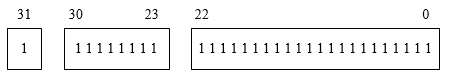
\includegraphics[scale=1]{Binary32.png}
				\end{center}
				\caption{Biểu diễn số thực 32 bits}	
					\label{fig:Bianry32}		
			\end{figure}
		\end{center}			

\subsection*{Bit dấu}
 Bit dấu của số dấu chấm động được biểu diễn bằng một bit. Nếu bit dấu bằng 1 số được biểu diễn là số âm, nếu là 0 số được biểu diễn là số dương. \\
 
 \subsection*{Phần Mantissa}
 	Phần mantissa rất hữu ích cho việc biểu diễn số thực dấu chấm động. Lấy ví dụ $-3.154 \times 10^5$, bit sign là số âm (1), phần mantissa là 3.154 và expoment là 5. Phần thập phân của mantissa là tổng mỗi chữ số nhân với cơ số 10 số mũ của 10 theo vị trí lần lượt từ trái qua phải, đằng sau dấu phẩy:
 	
 		$.154$ = $\frac{1}{10} + \frac{5}{100} + \frac{4}{1000}$
 		
 	Số thực dấu chấm động ở dạng nhị phân rát đơn giản. Ví dụ, trong số $+11.1011 \times 2^3$, bit sign là số dương (0), phần mantissa 11.1011, và expoment là 3. Thần thập phân của mantissa là tổng mỗi chữ số nhân với cơ số 2 số mũ của 2 lần lượt là vị trí của từng chữ số sau dấu phẩy:
 	
 		$.1011 = \frac{1}{2}+ \frac{0}{4} + \frac{1}{16}$
 		
 		Có thể tính phần thập phân của mantissa 1011 bằng cách chia cho $2^4$. Giá trị có được là $11/16 = 0.6875$. Kết hợp với phần nguyên của ví dụ là $11.$ tương ứng là 3, cơ số 10 của ví dụ này là 3.6875. Dưới đây là một số ví dụ khác:
 		\begin{longtable}{|l|l|l|}
 			\hline 
 				Nhị phân dấu chấm động & Cơ số 10 của phần thập phân & Cỏ số 10 \\
 			\hline
 			\hline
 				11.11 & 3 $\frac{3}{4}$ & 3.75\\
 			\hline
 				0.0000000000000000000001 & $\frac{1}{8388608}$ & 0.000001192092895578125 \\
 			\hline
 		\end{longtable}
 		
 		Bảng ~\ref{tb:VDBinary} trình bày một số ví dụ đơn giản cách biểu diễn phần thập phân của số thực dấu chấm động, giá trị cơ số 10 của mỗi giá trị:
 		\begin{longtable}{|l|l|l|}
 			\hline
 				Nhị phân & Phần thập phân & Giá trị cơ số 10 \\
 			\hline
 			\hline
 				.1 & $\frac{1}{2}$ & .5 \\
 			\hline
 				.01 &$ \frac{1}{4}$ & .25 \\
 			\hline
 				.001 & $\frac{1}{8}$ & .125 \\
 			\hline
 				.0001 & $\frac{1}{16}$ &.0625 \\
 			\hline
 				.00001 & $\frac{1}{32}$ & .03125 \\ 			
 			\hline
 			\caption{Ví dụ biểu diễn số dấu chấm động}
 			\label{tb:VDBinary}
 		\end{longtable}
 		
 	 \subsection*{Phần Expoment}
 Phần expoment theo định dạng IEEE short real lưu trữ 8-bit là một số nguyên không dấu có số cơ sở là 127. Lấy lại ví ụ $1.101 \times 2^5$ có expoment là 5, số 5 này được cộng với số cơ sở 127 được tổng là 132 biểu diễn ở dạng nhị phân số nguyên là 10000100. Bảng ~\ref{tb:VDEx} đưa ra một số ví dụ về điều chỉnh phần expoment và được biểu diễn sang số nhị phân:
 	\begin{longtable}{|l|l|l|}
 		\hline
 			Expoment & Điều chỉnh & Số nhị phân \\
 		\hline
 		\hline
 			+10 & 137 & 10001001 \\
 		\hline
 			0 & 127 & 01111111 \\
 		\hline
 			-5 & 122 & 01111010 \\
 		\hline
 			+128 & 255 & 11111111 \\
 		\hline
 			-127 & 0 & 00000000 \\ 		
 		\hline
 			\caption{Ví dụ về expoment}
 			\label{tb:VDEx}
 	\end{longtable}
 	
 	Giá trị expoment sau khi điều chỉnh không được âm. Giá trị nhất của số expoment là 128 khi được công thêm số mũ cơ sở (127) là 255. Đây là số lớn nhất mà 8-bit có thể biểu diễn được. Phạm vi của số mũ trong định dạng short real là $1.0 \times 2^{-127} $tới $1.0 \times 2^{+128}$
\subsection*{Biểu diễn Mantissa về định đạng chuẩn}
	Trước khi số thực dấu chấm động được mã hóa nhị phân lưu chính xác giá trị của số đó, phần mantissa cần phải đưa về dạng chuẩn. Việc xử lý này dựa trên thao tác toán học số thực dấu chấm động. Ví dụ, để biểu diễn số 1234.567 sang dạng chuẩn là 1.234567 $\times 10^3$ bằng cách dịch chuyển dấu phẩy sang trái đồng thời nhân với cơ số 10 số mũ tăng lên theo vị trí mỗi số dịch qua. Số mũ tăng lên khi được dịch qua trái, và giảm xuống khi dịch qua phải.
	
	Tương tự như vậy khi biểu diễn số thực sang số nhị phân. Lấy ví dụ 1101.101 đưa về dạng chuẩn sẽ là 1.101101 $\times 2^3$ bằng cách dịch dấu chấm sang trái ba số đồng thời nhân với  $2^3$. Bảng ~\ref{tb:VDMa} đưa ra một số ví dụ: \\ \\
	
	\begin{longtable}{|l|l|l|}
		\hline
			Giá trị nhị phân & Dạng chuẩn & Số Expoment \\
		\hline
		\hline
			1111.001 & 1.111001 & 3 \\
		\hline
			.0000101 & 1.01 & -5 \\
		\hline
			1.1010 & 1.1010 & 0 \\
		\hline
			100011000.0 & 1.000110000 &  8\\
		\hline
			\caption{Ví dụ biểu diễn số mantissa}
			\label{tb:VDMa}
	\end{longtable}

\subsection*{Biểu diễn nhị phân theo chuẩn IEEE}
	Khi đã biểu diễn được bit sign, phần expoment và phần mantissa theo dạng chuẩn. Biểu diễn các bit theo thứ tự như hình ~\ref{fig:Bianry32}. Ví dụ lấy giá trị nhị phân là 1.101 $\times 2^0$ có bit dấu là 0 (số dương), số mũ hiện là 0 nhưng được điều chỉnh bằng cách cộng với 127 (số cơ sở theo định dạng shorl real)  là 127 biểu diễn ở mã nhị phân là 01111111. Số "1" ở phía bên trái cao nhất của phần mantissa (1.101) được loại bỏ lấy phần sau dấu phẩy là 101. Theo thứ tự bit định dạng  IEEE shorl real là 1 01111111 1010000000000000000000. Bảng ~\ref{tb:VDIEEE} trình bày một số ví dụ:
	\begin{longtable}{|l|l|l|}
	\hline
		Giá trị nhị phân & Expoment & Sign, Expoment, Mantissa\\
	\hline
	\hline
		-1.101 & 127 & 1 01111111 10100000000000000000000 \\
	\hline
		+1101.1110 & 130 & 0 10000010 11100000000000000000000 \\
	\hline
		-0.000101 & 124 & 1 01111100 01000000000000000000000 \\
	\hline
		+1111110001.0 & 136 & 1 10001000 11111100010000000000000 \\
	\hline
		+0.0000001101011& 120 & 1 01111000 10101100000000000000000 \\
	\hline
		\caption{Ví dụ chuản IEEE}
		\label{tb:VDIEEE}
	\end{longtable}	

\newpage
\fancyhead[R]{\slshape PHỤ LỤC}
\begin{center}
	\begin{huge}
			\textbf{PHỤ LỤC 2}\\
			\textit{Công cụ Ollydbg}
	\end{huge}
\end{center}

\subsection*{Giới thiệu}
	OllyDbg là một công cụ sử dụng hợp ngữ trên nền Windows 32-bit chú trọng đến việc phân tích mã nhị phân. Công cụ dò xét các thanh ghi, nhận diện các thao tác với câu lệnh assmebly, các lời gọi hàm API, hằng số, chuỗi, từ khóa chuyển câu lệnh, cũng như chỉ ra địa chỉ thao tác từ tập tin và các thư viện. Công cụ ollydbg hoàn toàn miễn phí và đầy đủ chức năng, không có giới hạn thời gian sử dụng, nhưng có thông tin đăng ký với tác giả như ở các dạng phần mềm dùng thử. Các phiên bản hiện tại của OllyDbg không thể thao tác được các tập tin biên dịch cho các bộ vi xử lý 64-bit.
\subsection*{Thao tác}
Hình~\ref{fig:GiaoDienOllydbg} thể hiện giao diện chính của Ollydbg
	\begin{center}
			\begin{figure}[htp]
				\begin{center}
					\includegraphics[scale=0.75]{GiaoDienollydbg.png}
				\end{center}
				\caption{Giao diện công cụ Ollydbg}	
					\label{fig:GiaoDienOllydbg}		
			\end{figure}
		\end{center}		

File đầu vào của công cụ Ollydbg là một file thực thi có đuôi file là \textit{".exe"}. Để mở file, theo đường dẫn File->Open để chon nơi lưu file sau đó Click Open. Ngoài ra có thể thao tác click vào biểu tượng thư mục như hinh ~\ref{fig:OpenOllydbg} để mở file.
		\begin{center}
			\begin{figure}[htp]
				\begin{center}
					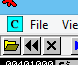
\includegraphics[scale=1]{OpenOllybdg.png}
				\end{center}
				\caption{Mở file trong Ollydbg}	
					\label{fig:OpenOllydbg}		
			\end{figure}
		\end{center}		
Khi mở một flie thực thi sẽ có giao diện như hình ~\ref{fig:VDOllydbg}
	\begin{center}
			\begin{figure}[htp]
				\begin{center}
					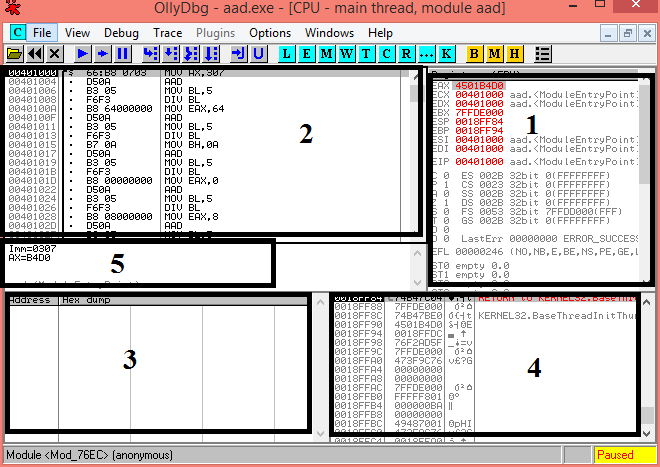
\includegraphics[scale=0.75]{VDOllydbg.png}
				\end{center}
				\caption{Ví dụ Ollydbg}	
					\label{fig:VDOllydbg}		
			\end{figure}
		\end{center}		
		
Giao diện khi mở một file thực thi có 5 cửa xổ
	
	\begin{itemize}
		\item[1] Cửa số thanh ghi (Registers): đây là cửa số chứa thông tin chi tiết về các thanh ghi như eax, ebx, ecx v….v…..Các cờ trạng thái cũng được quản lý tại cửa sổ này.
		\item[2] Cửa số giả mã assembly (Disassembler): cửa sổ này cho thấy các đoạn code của chương trình ở dạng ngôn ngữ assembly, và đồng thời tại cửa sổ này người dùng cũng có thể chú thích cho từng từng dòng mã assembly .
		\item[3] Cửa số giải mã giá trị (Dump): cửa sổ cho thấy bộ nhớ hiện tại của chương trình theo 2 dạng là hex và Ascii đồng thời cho phép chỉnh sửa bộ nhớ.
		\item[4] Cửa số stack:  mọi câu lệnh trước khi được thực hiện phải được nạp vào Stack.
		\item[5] Cửa số thông báo toán hạng (Tip):  Khi chương trình đang ở tại một dòng code nào đó trong quá trình debug ,  Olly sẽ cho thấy thông tin chi tiết về dòng code đó. Ví dụ  : nếu đang debug ở dòng lệnh \textit{ “ mov eax , dword ptr [123]”} . Thì cửa sổ này sẽ cho biết được giá trị hay con số nào đang được lưu giữ tại [123].
		\end{itemize}
	
	\subsubsection*{Cửa số Register}	
	Hình ~\ref{fig:OllydbgReg} thể hiện cửa số Register chứa các biến môi trường được dùng để thao tác với  mỗi câu lệnh.
	\begin{center}
			\begin{figure}[htp]
				\begin{center}
					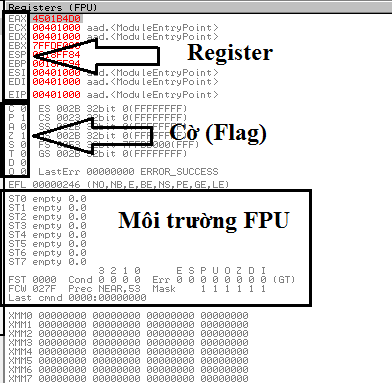
\includegraphics[scale=0.75]{OllydbgReg.png}
				\end{center}
				\caption{Cửa sổ Register trong Ollydbg}	
					\label{fig:OllydbgReg}		
			\end{figure}
		\end{center}		
		
		Cửa số này sẽ cung cấp rất nhiều thông tin trong quá trình chúng ta làm việc với Ollydbg. Các biến EAX, EBX, ECX, EDX, ... thể hiện các thanh ghi xử lý số nguyên. Các biến cờ C, P, A, Z... thay đổi trong quá trình thao tác với các câu lệnh số nguyên. Các biến ST0, ST1, ST2, ... FCW, FSW biểu diễn stack thanh ghi dữ liệu FPU, thanh ghi điều khiển FPU, thanh ghi trạng thái FPU.
		
	\subsubsection*{Cửa số Disassembler}
	Hình ~\ref{fig:OllydbgDisasm} thể hiện cửa sổ Disassembler, biểu diễn các câu lệnh assembly của chương trình đầu vào.. 
		\begin{center}
			\begin{figure}[htp]
				\begin{center}
					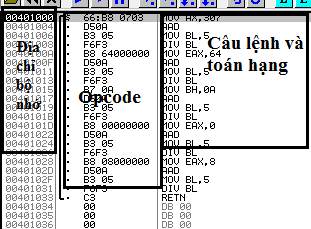
\includegraphics[scale=1]{OllydbgDisasm.png}
				\end{center}
				\caption{Cửa sổ Disassembler trong Ollydbg}	
					\label{fig:OllydbgDisasm}		
			\end{figure}
		\end{center}		
		
		Khi muốn debug một chương trình, cần phải load file thực thi của chương trình đó vào trong Ollydbg. Các chương trình mà đã được load vào Ollydbg là những chương trình có thể được code bằng những ngôn ngữ khác nhau như : VB, VC++, Borland Delphi hay MASM nhưng tại cửa sổ này toàn bộ code của chương trình sẽ được list ra dưới dạng các mã ASM. Ollydbg tiến hành phân tích chương trình và thể hiện chương trình dưới dạng assembly ở cửa số này đồng thời cung cấp tên câu lệnh assembly cùng với các toán hạng. Cho biết địa chỉ câu lệnh đang ở đâu trong bộ nhớ cùng mã opcode của câu lệnh assembly đang hiện hành. 
	
		\newpage
		\subsubsection*{Cửa sổ stack}
		Trước tiên sẽ đi tìm hiểu sơ qua về Stack. Đây là nơi lưu trữ tạm thời các dữ liệu và địa chỉ, nó là một cấu trúc dữ liệu một chiều. Các phần tử được cất vào và lấy ra từ một đầu của cấu trúc này, tức là nó được xử lý theo phương thức “vào trước, ra sau” (LIFO : Last In First Out). Phần tử được cất vào cuối cùng gọi là đỉnh của Stack. Có thể hình dung Stack như là một chồng đĩa, chiếc đĩa được đặt lên cuối cùng sẽ nằm trên đỉnh và chỉ có nó mới có thể được lấy ra đầu tiên. Hai thanh ghi chính làm việc với Stack là ESP và EBP. Theo mặc định trong Olly, Stack được biểu diễn theo thanh ghi ESP tuy nhiên ta có thể luân chuyển qua lại giữa ESP và EBP bằng cách nhấn chuột phải và chọn như hình~\ref{fig:OllydbgStack}
		\begin{center}
			\begin{figure}[htp]
				\begin{center}
					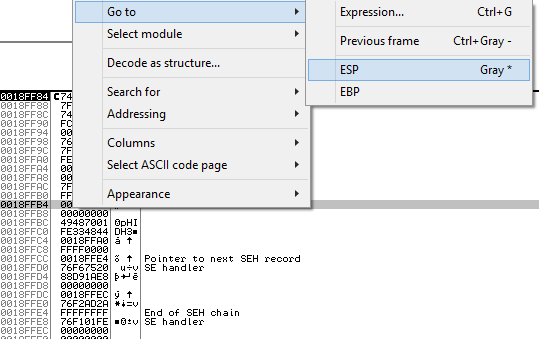
\includegraphics[scale=1]{OllydbgStack.png}
				\end{center}
				\caption{Cửa sổ Stack trong Ollydbg}	
					\label{fig:OllydbgStack}		
			\end{figure}
		\end{center}				
	
	\newpage	
	\subsubsection*{Cửa sổ Dump}
	Đây là cửa số hiện thị nội dung của bộ nhớ hoặc file. Ta có thể chọn nhiều định dạng khác nhau để biểu diễn nội dung của memory trong cửa số này : byte, text, integer, float, address, disassembly hoặc PE Header. Cửa sổ này cho phép chúng ta tìm kiếm cũng như  thực hiện các chức năng chỉnh sửa, thiết lập các Break points v..v... được thể hiện trong hình ~\ref{fig:OllydbgDump}.
	\begin{center}
			\begin{figure}[htp]
				\begin{center}
					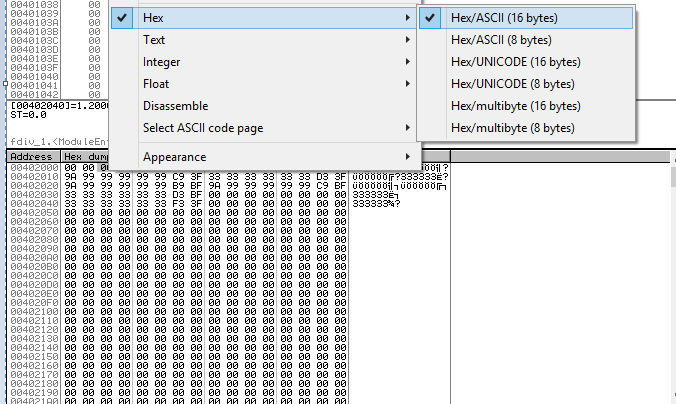
\includegraphics[scale=1]{OllydbgDump.png}
				\end{center}
				\caption{Cửa sổ Dump trong Ollydbg}	
					\label{fig:OllydbgDump}		
			\end{figure}
		\end{center}		
	
	\newpage
	\subsubsection*{Chức năng}
	Tiếp theo sẽ giới thiệu qua chức của từng nút trên thanh công cụ Ollydbg(hình ~\ref{fig:OllydbgBut} )
		\begin{center}
			\begin{figure}[htp]
				\begin{center}
					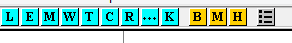
\includegraphics[scale=1]{OllydbgBut.png}
				\end{center}
				\caption{Chức năng trong Ollydbg}	
					\label{fig:OllydbgBut}		
			\end{figure}
		\end{center}		
		
		\begin{itemize}
			\item[•] 	Nút L dùng để mở cửa sổ Log của Olly, cửa sổ thể hiện những thông tin mà Olly ghi lại. Theo mặc định thì cửa số này sẽ lưu các thông tin về các module, import library hoặc các Plugins được load cùng chương trình tại thời điểm đầu tiên khi ta load chương trình vào Olly. Bên cạnh đó cửa sổ này cũng ghi lại các thông tin về các Break points mà chúng ta đặt trong chương trình.
			\item[• ] Nút E dùng để mở cửa sổ Executables, cửa sổ này thể hiện danh sách những file có khả năng thực thi được chương trình sử dụng như file exe, dlls, ocxs , v..v.. 
			\item[•] Nút M dùng để mở cửa sổ Memory, cửa sổ này sẽ cho chúng ta thông tin về bộ nhớ đang được sử dụng bởi chương trình.
			\item[• ] 	Nút T dùng để mở cửa sổ Threads, cửa sổ này liệt kê các Threads của chương trình.
			\item[•]  	Nút W dùng để mở cửa sổ Windows.
			\item[• ] 	Nút H dùng để mở cửa sổ Handles.
			\item[• ]  Nút \/ để mở cửa sổ Patches, cửa sổ này sẽ cho chúng ta các thông tin về những thông tin đã edit trong chương trình.
			\item[•]  Nút K để mở cửa sổ Call Stack, hiển thị một danh sách các lệnh call mà chương trình  đã thực hiện khi  Run bằng F9 và dùng F12 để tạm dừng chương trình.
			\item[•]  Nút B để mở cửa sổ Break Points, cửa sổ này sẽ hiển thị tất cả các BPs mà đã đặt trong chương trình. Tuy nhiên nó chỉ hiện thị các BPs được set bằng cách nhấn F2, còn các dạng BPs khác như : hardware breakpoint hoặc memory breakpoints thì không được liệt kê ra ở phụ lục này.
			\item[•] Nút R để mở cửa sổ References, cửa sổ này là kết quả khi hực hiện chức năng Search trong Ollydbg.	
		\end{itemize}		
	
	\subsubsection*{Phím tắt}
	\textbf{F7 : } Khi nhấn F7 sẽ thực thi từng dòng lệnh 1. Nếu trong quá trình thực thi mà gặp lệnh Call thì sẽ đi vào trong lòng của lệnh Call đó và thực thi từng câu lệnh trong lệnh Call này cho đến khi gặp lệnh Retn để trở lại chương trình chính, tức là câu lệnh tiếp theo sau lệnh Call.\\
	
		\textbf{F8 :} Cũng tương tự như F7 nhưng có 1 điểm khác biệt trong quá trình thực thi từng câu lệnh, nếu như gặp lệnh Call nó bỏ qua không cần quan tâm các lệnh bên trong lệnh Call mà thực thi luôn lệnh Call đó và dừng lại tại câu lệnh tiếp theo dưới lệnh Call.\\
		
		\textbf{F2 :} Đặt một Break point trong chương trình. Vậy Break point là gì , đơn giản nó chỉ là việc chúng ta tạo 1 điểm ngắt trong chương trình theo một điều kiện nào đó để khi thực thi chương trình, nếu thỏa điều kiện mà chúng ta đặt ra thì chương trình sẽ dừng lại tại vị trí mà chúng ta đã đặt BP.\\
		 
		\textbf{F9 :}  Cho phép thực thi chương trình trong chế độ Debug, tương tự như việc chúng ta nhấp đúp chuột vào chương trình để thực thi nó. Tuy nhiên khác với việc nhấp đúp chuột, nếu chúng ta nhấn F9 thì Olly sẽ tìm xem có BP nào được Set hay không, chương trình có hiện thị ra các Exception gì không, hay nếu chương trình có cơ chế chống Debug thì nó sẽ ngắt  ngay lập tức. Nếu như không có bất kì cản trở nào thì chương trình sẽ Run hoàn toàn và trên status bar của Olly sẽ báo cho chúng ta biết điều này.
		
		\textbf{F12 :} Tạm dừng chương trình lại.

\newpage
\fancyhead[R]{\slshape PHỤ LỤC}
\begin{center}
	\begin{huge}
			\textbf{PHỤ LỤC 3}\\
			\textit{Công cụ MASM32}
	\end{huge}
\end{center}

	\subsection*{Giới thiệu}
	Có hai loại trình biên dịch được sử dụng để biên dịch chương trình hợp ngữ (từ tập lệnh hợp ngữ của các vi xử lý họ Intel) sang chương trình thực thi: Trình biên dịch hợp ngữ 16 bít, MASM (Macro Assembler), được sử dụng để dịch thành các chương trình chạy trên nền hệ điều hành 16 bít MS-DOS; Trình biên dịch hợp ngữ 32 bít, MASM32 (Macro Assembler 32 bít), được sử dụng để dịch thành các chương trình chạy trên nền hệ điều hành 32 bít  MS-Windows. Trong quá trình làm luận văn, công cụ MASM 32 bit được sử dụng để tạo các test-case, hiện thực các câu lệnh.
	
	\subsection*{Thao tác}
	Để viết một chương trình bằng MASM ta sử dụng QEDITOR.exe trong thư mục MASM có giao diện như hình ~\ref{fig:MASM}
	\begin{center}
			\begin{figure}[htp]
				\begin{center}
					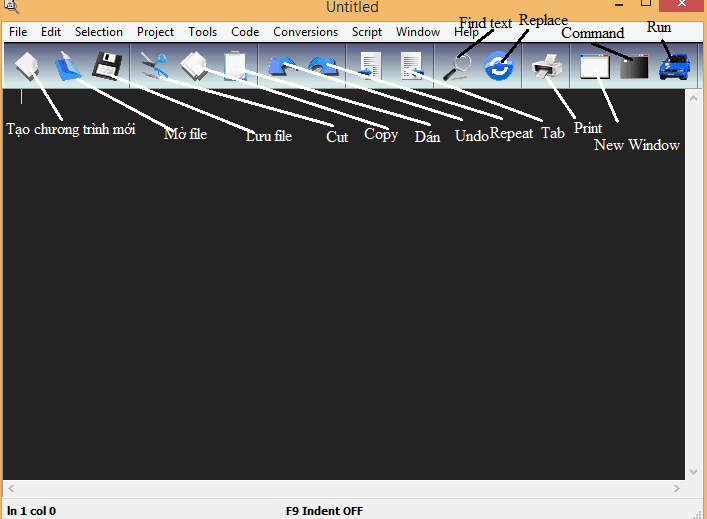
\includegraphics[scale=0.5]{MASMGiaoDien.png}
				\end{center}
				\caption{Giao diện công cụ MASM32}	
					\label{fig:MASM}		
			\end{figure}
		\end{center}			
	
	
	Trên thanh status bar có các chức năng: Tạo chương trình mới, mở file, lưu file, cut, copy, dán, undo, repeat, tab, find text, replace, print, command, new window, run.\\

	Trước khi biên dịch chương trình cần phải lưu chương trình trước, và trong quá trình làm việc nếu có thay đổi phải lưu trước khi biên dịch vì MASM32 không có cơ chế tự lưu những thay đổi như VC hay VB, và một điều nữa cần chú ý là chức năng Undo trong Masm chỉ cho phép undo 1 hành động vì vậy khi có nhiều thay đổi mà người dùng nghĩ có thể phải undo thì nên save trước , nếu cần phục hồi lại thì exit và không save thì nó sẽ ở trạng thái ở lần save cuối cùng. Ví dụ nếu đã có mã code và bây giờ cần biên dịch vào Menu item: Project, trong menu Project có các mục sau: 
		\begin{itemize}
			\item[•] Compile Resource File: biên dịch file resource, file resource có phần mở rông *.rc file này chứa các tàì nguyên như Icon, DialogBox, Bitmap... mà chương trình sử dụng. 
		\item[•] Assemble Asm file: Tạo file *.Obj từ file .asm. 
		\item[•]  Link Obj: từ file Obj link tới các tài nguyên cần thiết để tạo file exe.
		 \item[•]  Assemble \& Link: thực hiện cả hai bước trên , việc này sẽ tạo sự thuận tiện cho người lập trình, không phải tốn công thực hiện qua hai bước mới tạo nên file .exe
		 \item[•]  Build all: Chức năng này có tác dụng biên dịch cả file resource, và tạo file .exe. Chức năng này được sử dụng khi  có thay đổi những tài nguyên ở file resource. Còn nếu chỉ thay đổi về code trong chương trình thì nên sử dụng Assemble \& link, nó sẽ rút ngắn thời gian biên dịch.
		 \item[•]  Run Makeit.bat: nếu muốn có một file Makeit.bat và muốn sử dụng nó để biên dịch thay vì xài những tùy chọn biên dịch mặc định của MASM. Cũng với những chức năng trên nhưng có thêm console thì khi chạy chương trình ccòn kèm theo một cửa sổ dòng lệnh.
		   \item[•]  Run Program: để chạy thử chương trình sau khi biên dịch. 
		\end{itemize}
		



\newpage
\fancyhead[R]{\slshape PHỤ LỤC}
\begin{center}
	\begin{huge}
			\textbf{PHỤ LỤC 1}\\
			\textit{Bảng công việc}
	\end{huge}
\end{center}

	\begin{longtable}{|l|m{13cm}|}
		\hline
			Tuần & Nội dung công viêc \\
		\hline
		\hline
			2/3 - 8/3	& Thực hiện test case với số câu lệnh hiện có trong BE-PUM\\
		\hline	
			16/3 - 5/4&	Nghiên cứu tài liệu về câu lệnh xử lý số nguyên, đồng thời hỗ trợ anh Hải trong một số công việc.\\
		\hline	
			5/4 - 12/4&	Mô phỏng câu lênh CMOVcc\\
		\hline	
			13/4 - 17/5	&Mô phỏng câu lênh  BSWAP, XADD, CMPXCHG, CMPXCHG8B, CWD/CDQ, CBW, CWDE, SHRD, SHRL, RCL, RCR,  BT, BTS, ....\\		
		\hline	
			18/5 -31/5	&Thực hiện test với các câu lệnh đã được mô phỏng\\
		\hline	
			1/6 - 14/6	&Viết  và hoàn thiện báo cáo  thực tập tốt nghiệp.\\	
		\hline	
			3/8 - 23/8&	Thực hiện test với các câu lệnh xử lý số nguyên.\\
		\hline	
			24/8 - 13/9&	Nghiên cứu tài liệu về FPU, đồng thời hỗ trợ anh Hải trong một số công việc.\\
		\hline	
			14/9 - 27/9	&Hiện thực số thực. Gặp vấn đề trong biểu diễn số thực.\\
		\hline	
			28/9 - 4/10&	Giải quyết vấn đề biểu diễn số thực.\\
		\hline	
			5/10 - 11/10&	Biểu diễn số thực dạng nhị phân, lưu trữ được vào trong stack thanh ghi.\\
		\hline	
			12/10 - 18/10&	Mô phỏng các câu lệnh FADD, FADDP, FIADD, FSUB, FSUBP, FSUBR, FSUBRP, FISUB, FISUBR, FMUL, ..\\
		\hline	
			19/10 - 25/10&	Mô phỏng các câu lệnh  FDIVRP, FIDIVR, FABS, FCHS, FSQRT, FPREM, FPREM1, FRNDINT, FXTRACT, FSIN, FCOS, FSINCOS,..\\
		\hline
			26/10 - 15/11	&Mô phỏng các câu lệnh FCOM, FCOMP, FCOMPP, FUCOM, FUCOMP, FUCOMPP, FICOM,  FTST, FXAM...\\		
		\hline	
			16/11 - 29/11&	Tiến hành test để kiểm tra sự chính xác của các câu lệnh được mô phỏng.\\
		\hline	
			30/11 - 6/12	&Viết báo cáo luận văn.\\
		\hline	
			7/12 - 13/12	&Kiểm tra báo cáo luận văn.\\
		\hline	
			14/12 - 20/12&	Hoàn thiện báo cáo luận văn.\\
		\hline
			\caption{Bảng kế hoạch nghiên cứu hiện thực câu lệnh assembly}
	\end{longtable}

\newpage

\fancyhead[R]{\slshape TÀI LIỆU THAM KHẢO}
\begin{thebibliography}{}

\bibitem{cfg-def}
Frances E. Allen. \emph{Control flow analysis}. SIGPLAN Notices 5 (7): 1–19. July 1970.


\end{thebibliography}

\end{document}



